\documentclass{layout/tudelft-report}

%% Setting up the bibliography
\usepackage{biblatex}
\addbibresource{master_thesis.bib}

%% Additional packages and commands
\setlist{itemsep=-2pt} % Reducing white space in lists slightly
\renewcommand{\deg}{\si{\degree}\xspace} % Use \deg easily, everywhere

%%%%%%%%%%%%%%%%%%%%%%%%%%%%%
%%%%% Begin of document %%%%%
%%%%%%%%%%%%%%%%%%%%%%%%%%%%%

\begin{document}

%% Roman page numbering
\frontmatter

%% Defining the main parameters
\title{Stability guarantees in variable impedance control for rigid robotics manipulators in contact with (semi)-rigid environments}
\subtitle{HOW TO GUARANTEE STABLE VARIABLE IMPEDANCE CONTROL AT ALL TIMES}
\author{Rick Staa}
\subject{ME51010: ME-BMD Literature Report}
\affiliation{Delft University of Technology}

% Source: https://www.franka.de/
\coverimage{figures/cover_cropped.jpg} % Aspect ratio of 2:3 (portrait) recommended

\definecolor{title}{HTML}{4884d6} % Color for title

\makecover

\begin{titlepage}

\begin{center}

%% Print the title
{\makeatletter
\largetitlestyle\fontsize{45}{45}\selectfont\@title
\makeatother}

%% Print the subtitle
{\makeatletter
\ifdefvoid{\@subtitle}{}{\bigskip\titlestyle\fontsize{20}{20}\selectfont\@subtitle}
\makeatother}

\bigskip
\bigskip

by

\bigskip
\bigskip

%% Print the name of the author
{\makeatletter
\largetitlestyle\fontsize{25}{25}\selectfont\@author
\makeatother}

\bigskip
\bigskip

%% Print table with names and student numbers
\setlength\extrarowheight{2pt}
\begin{tabular}{lc}
    Student Name & Student Number \\\midrule
    Rick Staa & 4511328 \\
\end{tabular}

\vfill

%% Print some more information at the bottom
\begin{tabular}{ll}
    Main Instructor: & Prof.dr.ir. M. (Martijn) Wisse \\
    Secondary Instructor: & Dr. W. (Wei) Pan \\
    Project Duration: & March, 2022 - March, 2023 \\
    Faculty: & Cognitive Robotics, Delft
\end{tabular}

\bigskip
\bigskip

%% Add a source and description for the cover and optional attribution for the template
\begin{tabular}{p{15mm}p{10cm}}
    Cover: & Picture of Franka Research 3 robot from https://www.franka.de/\\
    % Feel free to remove the following attribution, it is not required - still appreciated :-)
    Style: & TU Delft Report Style, with modifications by Daan Zwaneveld
\end{tabular}

\end{center}

%% Insert the TU Delft logo at the bottom of the page
\begin{tikzpicture}[remember picture, overlay]
    \node[above=10mm] at (current page.south) {%
        
\includegraphics{layout/tudelft/logo-black}
    };
\end{tikzpicture}

\end{titlepage}

% \chapter*{Preface}
\addcontentsline{toc}{chapter}{Preface}

\emph{A preface...}

\begin{flushright}
{\makeatletter\itshape
    \@author \\
    Delft, \monthname{} \the\year{}
\makeatother}
\end{flushright}

\chapter*{Abstract}
\addcontentsline{toc}{chapter}{Abstract}

\emph{A summary... blabla}


\tableofcontents
\listoffigures
\listoftables
\tcblistof[\chapter*]{ex}{List of Examples}
\tcblistof[\chapter*]{th}{List of Theorems}
\tcblistof[\chapter*]{def}{List of Definitions}

\chapter*{Nomenclature}
\addcontentsline{toc}{chapter}{Nomenclature}

This chapter contains abbreviations and symbols used throughout this report. It only includes abbreviations and symbols specific to this report or ones with ambiguous definitions. Please check out \cite{ListMathematicalSymbols2022} for a list of standardized math symbols.

\section*{Abbreviations}

\begin{longtable}{p{2.5cm}p{8cm}}
    \toprule
    Abbreviation & Definition                      \\
    \midrule\endhead % Abbreviations added alphabetically here:
    AS           & Asymptotically stable           \\
    CBF          & Control barrier function        \\
    CLF          & Control Lyapunov function       \\
    DMP          & Dynamic movement primitive      \\
    DOF          & Degree of freedom               \\
    DS           & Dynamic system                  \\   
    ES           & Exponential stable              \\
    GAS          & Globally asymptotically stable  \\
    GES          & Globally exponentially  stable  \\
    IL           & Imitation learning              \\
    IOS          & Input-Output stability          \\
    ISS          & Input-to-State stability        \\
    LfD          & Learning from demonstration     \\
    RL           & reinforcement learning          \\
    SISL         & Stable in the sense of Lyapunov \\
    UB           & Uniformly bounded               \\
    UUB          & Ultimately uniformly bounded    \\
    VIC          & Variable impedance control      \\
    ZSD          & Zero-state detectable           \\
    ZSO          & Zero-state observable           \\
    \bottomrule
\end{longtable}

\section*{Symbols}

\begin{longtable}{p{2.5cm}p{8cm}p{2.5cm}}
    \toprule
    Symbol              & Definition                              & Unit         \\
    \midrule\endhead % Latin symbols added alphabetically here:
    $V$                 & Lyapunov function                       &              \\
    $S$                 & Storage function                        &              \\
    $\mathcal{C}$       & Task space                              &              \\
    $\mathcal{J}$       & Joint space                             &              \\
    $x$                 & Position                                & [$m$]        \\
    $\bar{x}$           & Equilibrium point position              & [$m$]        \\
    $x_c$               & Impedance model reference position      & [$m$]        \\
    $x_d$               & Desired position                        & [$m$]        \\
    $x_e$               & Cartesian end effector position         & [$m$]        \\
    $q$                 & Generalized coordinates                 & [$rad$]      \\
    $M\left(.\right)$   & Manipulator inertia matrix              & [$kg/m^2$]   \\
    $C\left(.,.\right)$ & Manipulator Coriolis/centrifugal matrix & [$N$]        \\
    $f\left(.\right)$   & Manipulator friction force vector       & [$N$]        \\
    $g\left(.\right)$   & Manipulator gravity force vector        & [$N$]        \\
    $k\left(.\right)$   & Manipulator forward kinematics          &              \\
    $M_d$               & Desired inertia matrix                  & [$kg/m^2$]   \\
    $B_d$               & Desired damping matrix                  & [$Ns/m$]     \\
    $K_d$               & Desired stiffness matrix                & [$N\cdot m$] \\
    $J$                 & Geometric jacobian                      &              \\
    $J_A$               & Analytic jacobian                       &              \\
    \bottomrule
\end{longtable}


%% Arabic page numbering
\mainmatter

\chapter{Introduction}
\label{chapter:introduction}

As more and more robots move out of the factory into the real world, there is a growing need for robots that can safely work alongside humans or other robots \cite{sharkawySurveyApplicationsHumanRobot2021,zacharakiSafetyBoundsHuman2020,suomalainenSurveyRobotManipulation2021}. In order to do so, these robots must not only detect and avoid collisions \cite{haddadinRobotCollisionsSurvey2017, zacharakiSafetyBoundsHuman2020} but also safely interact with humans and the environment when a collision or a desired interaction occurs. Several researchers have proposed compliant or soft robots to prevent hard collisions and thus ensure safe interactions \cite{hughesSoftManipulatorsGrippers2016,douSoftRoboticManipulators2021}. Even though these robots are by no doubt safer than their rigid counterparts, they are more mechanically complex and unsuitable for tasks requiring high position accuracy, repeatability and effort \cite{douSoftRoboticManipulators2021}. As a result, researchers mainly resort to using rigid manipulators (sometimes with soft grippers) for robot manipulation tasks.

Although traditional position, velocity, and acceleration control algorithms, often used with rigid manipulators, achieve high precision and repeatability, they are stiff and not sensitive to force interaction. As a result, they are not suited for interacting with the environment because they may lead to large contact forces, resulting in unstable behaviour, damage or even accidents. On the other hand, effort control algorithms which can precisely regulate the contact force do not work in the absence of contact. To perform interaction tasks like manipulation, which contain both a free and contact phase, several researchers have used hybrid force/motion controllers \cite{raibertHybridPositionForce1981,ortenziHybridMotionForce2017}. These controllers divide the task space into a position-controlled (i.e., free) and force-controlled (constraint) subspace and switch between these spaces during the task. However, designing the switching behaviour of these hybrid controllers requires prior knowledge of the structure and geometry of the environment, which might not be available and is task-dependent also. Because of this, hybrid control algorithms cannot perform well in unstructured or dynamically changing environments.

Impedance control, in which the robot-environment interaction is modelled as a spring-damper system, is a better candidate. It can track a free-space trajectory while limiting the force applied to the environment when in contact. Traditionally, impedance controllers with constant parameters have been used \cite{hoganImpedanceControlApproach1985,hoganStableExecutionContact1987,calancaReviewAlgorithmsCompliant2016,songTutorialSurveyComparison2019,cheahLearningImpedanceControl1998,liHumanRobotCollaboration2013,heAdaptiveNeuralImpedance2015,liAdaptiveImpedanceControl2016,jamwalImpedanceControlIntrinsically2016,jungForceTrackingImpedance2004,ottPrioritizedMultitaskCompliance2015}. These controllers are passive and guarantee that the control never becomes unstable when controlling a passive robot in a passive environment. However, these controllers require accurate knowledge about the stiffness and location of the environment and can only attain a constant desired force. They can, therefore, not be used for dynamic force tracking or in uncertain or changing environments.

Variable impedance control (VIC) with time-varying impedance parameters provides a solution to this problem. By allowing the parameters to change over time, more complex tasks can be executed while also improving the robustness against uncertainties and changing environments. These variable impedance profiles can be implemented using adaptive or optimal controllers \cite{songTutorialSurveyComparison2019,erdenAssistingManualWelding2011,erdenRoboticAssistanceImpedance2016,leeForceTrackingImpedance2008,ikeuraOptimalVariableImpedance2002,medinaRisksensitiveInteractionControl2013,yangHumanlikeAdaptationForce2011} or learned from human demonstrations or through reinforcement learning (RL) \cite{buchliLearningVariableImpedance2011,rombokasTendondrivenVariableImpedance2013a,michelBilateralTeleoperationAdaptive2021,chenClosedLoopVariableStiffness2021,weiImpedanceControlUncertain2019,houVariableImpedanceControl2020,abu-dakkaVariableImpedanceControl2020,calinonLearningbasedControlStrategy2010,kronanderOnlineLearningVarying2012}. Although promising results have been obtained using these controllers in surgery \cite{ferragutiEnergyTankBasedInteractive2015, ferragutiTankbasedApproachImpedance2013}, human-robot interaction \cite{wuAdaptiveImpedanceControl2020,san-miguelAutomatedOffLineGeneration2022,sharifiImpedanceLearningBasedAdaptive2021} and welding and grinding tasks \cite{erdenAssistingManualWelding2011,erdenRoboticAssistanceImpedance2016,zhangLearningImpedanceRegulation2021,wangSafeOnlineGain2021}, it introduced one big problem. By varying the impedance parameters, the passivity property of the system no longer holds as energy can now be injected into the system, possibly making it unstable \cite{ferragutiTankbasedApproachImpedance2013}. Because unstable systems exhibit unpredictable and uncontrollable behaviour, they can not be deployed safely alongside humans or other robots.

Several solutions have been proposed in the relevant literature for keeping the control passive with varying impedance parameters. Although in recent years, multiple reviews have been conducted on the current state of the literature regarding VIC algorithms that robotic manipulators use for interaction tasks, they only briefly touch on this passivity issue \cite{suomalainenSurveyRobotManipulation2021,songTutorialSurveyComparison2019,abu-dakkaVariableImpedanceControl2020,al-shukaActiveImpedanceControl2018}. Therefore, this literature review aims to fill this gap by providing an extensive overview of the stability considerations and methods used in the current variable impedance literature for stable control of rigid robotics manipulators in contact with (semi)-rigid environments. Even though most of the techniques discussed in this literature review can also be applied to VIC in human-robot interaction (HRI) tasks, this is not the primary focus of this review. Readers interested in that subject can read the review done by \cite{sharifiImpedanceVariationLearning2021}. This review also does not consider stability problems caused by time delays in the control loop; such is often encountered during teleoperation. An extensive review on this subject can be found in \cite{farajiparvarBriefSurveyTelerobotic2020}.

This literature review is structured as follows: chapter \ref{chapter:method} depicts the methodology used for finding the relevant literature used in this review. After that, in chapter \ref{chapter:background}, essential concepts like VIC, Lyapunov stability and passivity are reviewed. The currently used techniques for ensuring closed-loop stability of classical variable impedance controllers are presented in chapter \ref{chapter:classical_variable_impedance}, while chapter \ref{chapter:learning_based_variable_impedance} describes the stability techniques used in learning-based controllers. Finally, chapter \ref{chapter:conclusion} discusses the current research trends and future challenges.


\chapter{Method}
\label{chapter:method}

% TODO: Make sure main papers are in here.

An extensive search of Web Of knowledge, Scopus, Semantic Scholar and Google Scholar was performed. During this search, keywords related to "variable impedance control", "stability", "passivity", "safety", and "robot manipulators" were used. In this search, articles before 2010 or related to "Human-Robot interaction", "teleoperation", "soft-robotics", "hydraulic joints", and "cable joints" were filtered out. A complete list of the keywords used can be found in appendix \ref{chapter:keywords}. In addition, the citation graphs of influential articles found in the first search \cite{ferragutiTankbasedApproachImpedance2013,khaderStabilityGuaranteedReinforcementLearning2020,kronanderStabilityConsiderationsVariable2016,khansari-zadehLearningStableNonlinear2011,mohammadkhansari-zadehLearningControlLyapunov2014} were inspected to check for missing articles. After these searches, the papers were manually inspected to check for relevance. The most important selection criteria were the significance of the contribution to stable variable impedance control and the technical quality of the work. If multiple studies presented a similar idea, the one with the highest technical quality was selected. If the quality was equal, the one published in a more prominent journal or with a higher citation count was selected.

\chapter{Background}
\label{chapter:background}

This chapter reviews some general concepts needed to understand the rest of the paper. First, the concept of stability is explained, and several methods used to prove stability are presented. This section is followed by a brief description of the dynamical model of the manipulator. Lastly, several indirect force control methods are introduced, such as impedance and admittance control.

\section{Stability}

The concept of stability is often explained using the example of a ball in a hilly landscape. A stable system can be represented by a ball placed in a valley. When this ball is disturbed (i.e., carried up the hill), it will always return to the lowest point, also called the equilibrium point, when released. When we now put this ball on top of a hill and disturb it (i.e., give it a push), we will see an unstable system instead. The ball will roll off the hill and never return without us carrying it up again. This stability can be local, only valid in a region around the equilibrium point or global and valid for all system states. In control theory, stability means that the control is guaranteed to always converges to a given setpoint while staying bounded in state space. This setpoint can be any arbitrary quantity like position, angle, velocity, effort, rotational speed, or voltage. In the case of a regularisation task, this setpoint can be static, but it can also move in time for trajectory tracking or manipulation tasks.

Multiple general methods have been designed to investigate the behaviour and stability of linear systems. Since a general closed-loop solution exists for a linear system, a simple eigenvalue analysis of this solution can be used to determine stability. The stability type and boundaries can be further investigated using frequency domain mathematical techniques like the Laplace transform, Fourier transform, z-transform, Bode plots, root locus, and Nyquist stability criterion \cite{bacciottiStabilityControlLinear2019}. Because a linear system only has one equilibrium point, it is always globally stable or unstable. On the other hand, no general closed-loop solution is available for nonlinear systems and determining stability is not trivial. Furthermore, nonlinear systems can also have multiple equilibrium points, meaning that stability can only be investigated locally around an equilibrium point and only under some conditions is global.

Lyapunov's stability theory, first introduced in 1892, provides a way to reason about the stability of equilibrium points of linear and nonlinear systems without solving the complete system behaviour. It consists of several notions of stability, fundamental theorems and methods that can be used to investigate the system's stability. Lyapunov's stability theory can be applied to both autonomous and non-autonomous systems. Below, several notions of stability for autonomous systems will be discussed, followed by methods that can be used to prove the stability of equilibrium points. After that, these notions and methods will be extended to unforced non-autonomous time-dependent systems. In doing so, the concept of boundedness, which is used for systems with no clear equilibrium point, and methods for dealing with perturbed systems are presented. Lastly, input-state stability and passivity will be introduced to investigate the stability of forced non-autonomous systems.

\subsection{Stability of autonomous systems}

\subsubsection{Stability notions}
% NOTE: The equations in this section come from \cite{khalilNonlinearSystems2002, mullerStabilityControlNonlinear2019}.

The introduction of Lyapunov's stability theory resulted in several new stability notions. The most used in the impedance literature are stability (and its absence, instability), asymptotic stability, and exponential stability.

%% FIGURE - Stability notions.
\begin{figure}
  \centering
  \begin{subfigure}{0.31\textwidth}
    \centering
    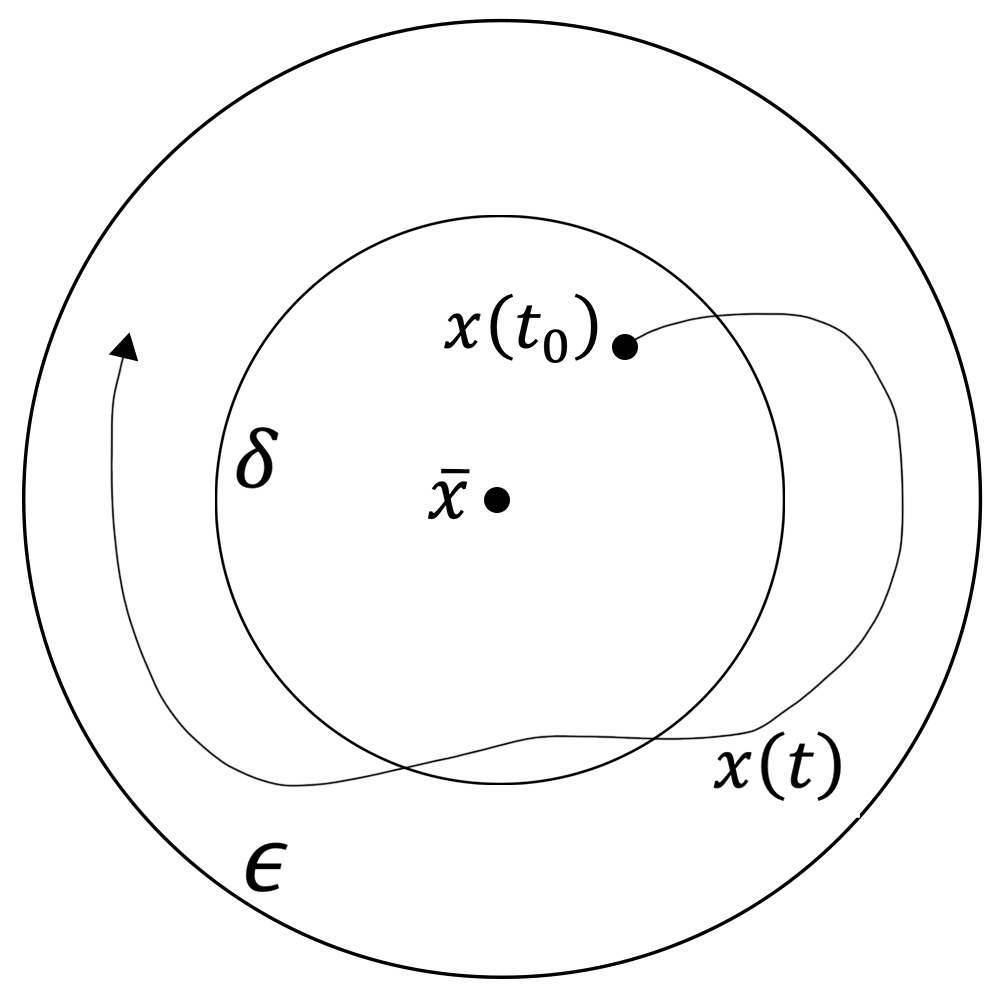
\includegraphics[width=\linewidth]{figures/figure-SISL.jpg}
    \caption{Stability in the sense of Lyapunov} \label{fig:SISL}
  \end{subfigure}
  \hspace*{\fill} % Maximize separation between the subfigures.
  \begin{subfigure}{0.31\textwidth}
    \centering
    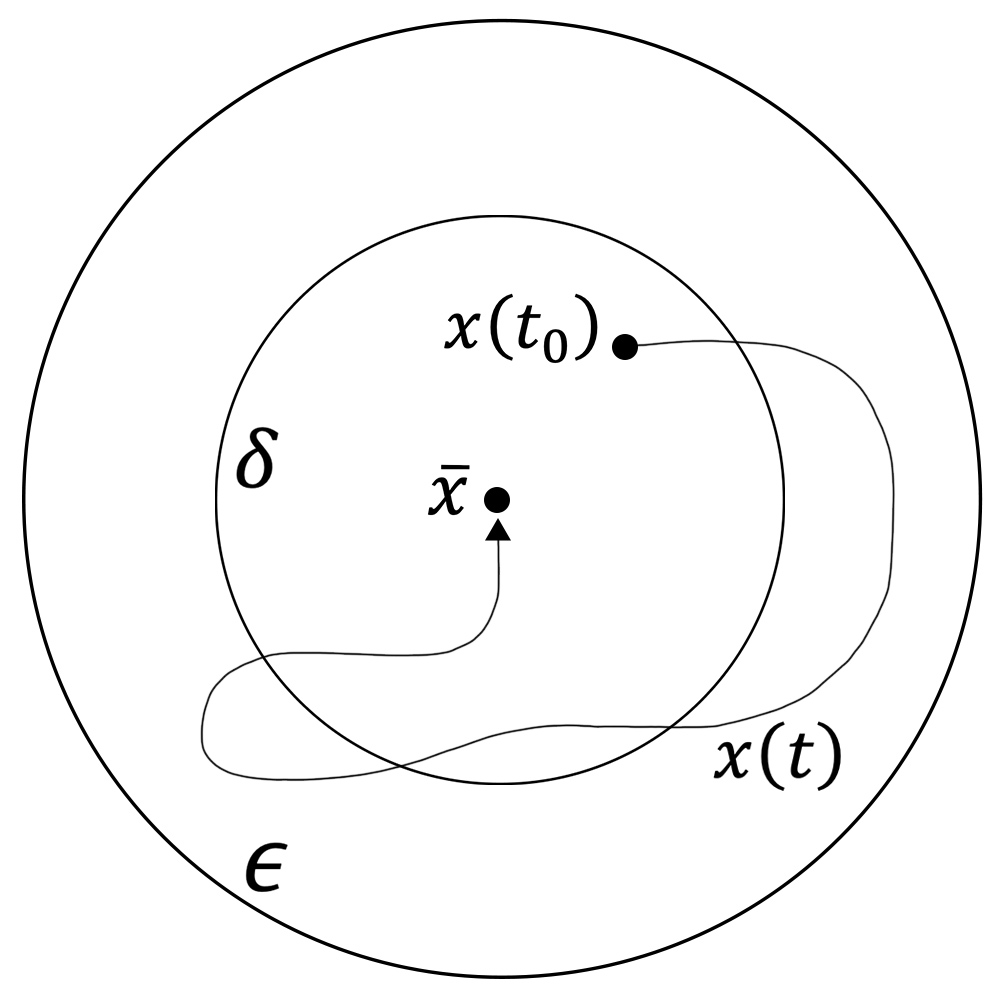
\includegraphics[width=\linewidth]{figures/figure-AS.jpg}
    \caption{Asymptotic stability} \label{fig:AS}
  \end{subfigure}
  \hspace*{\fill} % Maximize separation between the subfigures.
  \begin{subfigure}{0.31\textwidth}
    \centering
    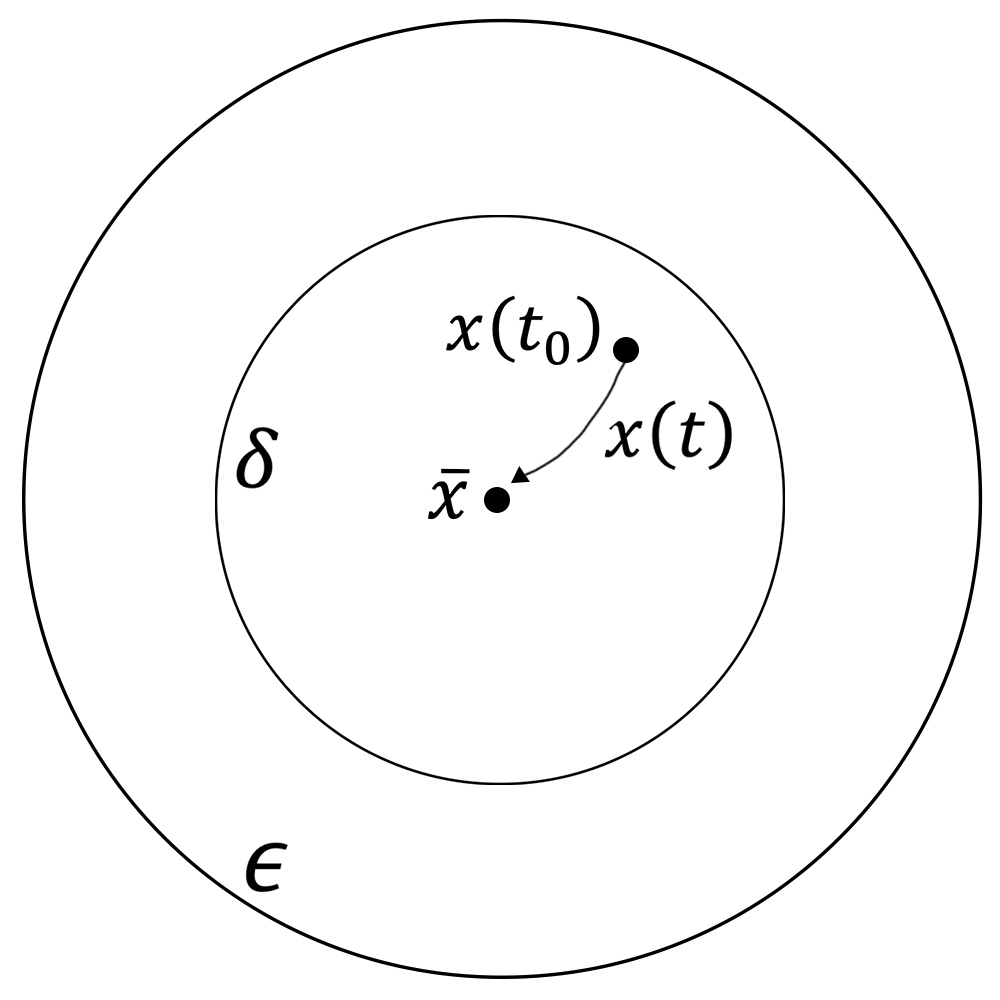
\includegraphics[width=\linewidth]{figures/figure-ES.jpg}
    \caption{Exponential stability} \label{fig:ES}
  \end{subfigure}

  \caption[Several notions of stability.]{Several notions of stability. In these figures, $\delta$, $\epsilon$ represent the start and end stability bounds, $\bar{x}$ the equilibrium point, and $x\left(t_0\right)$ and $x\left(t\right)$ the initial point and trajectory, respectively.} \label{fig:stability_notions}
\end{figure}

\paragraph{Stability in the sense of Lyapunov}

In Lyapunov's stability theory, stability is concerned with the trajectories' behaviour rather than the equilibrium point's stability. This notion of stability is handy since a noise or disturbance can always perturb a physical system from its equilibrium. Although, as shown in the following chapters, Lyapunov's theory can also be extended to work with specific non-autonomous systems, let us, for simplicity, consider the following autonomous nonlinear system:
\begin{equation} \label{eq:auto_nonlinear_system}
  \dot{x} = f\left(x\right),
\end{equation}
where $f : D \rightarrow\mathbb{R}^n$ is a locally Lipschitz map from a domain $D \subset \mathbb{R}^n$ into $\mathbb{R}^n$. An equilibrium point of this system $\bar{x}$ is \textbf{stable in the sense of Lyapunov (SISL)} if, for each $\epsilon > 0$, there exists some $\delta > 0$ such that:
\begin{equation}
  \left\| x\left(t\right) - \bar{x} \right\| < \epsilon, \quad \forall \; t \ge t_0,
\end{equation}
whenever $\left\| x\left(t_0\right) - \bar{x} \right\| < \delta$. Intuitively this means that any trajectory starting inside circle $\delta$ will never leave circle $\epsilon$ (see figure \ref{fig:SISL}). Since SISL is not a global condition, $\delta$ and $\epsilon$ should be chosen as small as possible to provide the most robust bounds. Logically, every system that does not adhere to these conditions is \textbf{unstable}.

\paragraph{Asymptotic stability}

A stricter notion of stability called asymptotic stability can be created by imposing some additional conditions. An equilibrium point $\bar{x}$ is \textbf{asymptotically stable (AS)} if:
\begin{itemize}
  \item It is SISL.
  \item Some $\delta > 0$ exists such that when $\left\| x\left(t_0\right) - \bar{x} \right\| < \delta, \quad \lim_{t \to \infty} \left\| x\left(t\right) - \bar{x} \right\| = 0$.
\end{itemize}
Intuitively this means that the trajectory will always converge to $\bar{x}$ if started inside circle $\delta$ (see figure \ref{fig:AS}). If $\delta = \infty$, the system is called \textbf{globally asymptotically stable (GAS)}.

\paragraph{Exponential stability}

Lastly, an equilibrium point $\bar{x}$ is \textbf{exponentially stable (ES)} with rate of convergence $\alpha$ if:
\begin{itemize}
  \item It is SISL.
  \item There exists a $M, \lambda > 0$ such that $\left\| x\left(t \right) \right\| \leq Me^{-\lambda\left(t-t_0 \right)}\cdot \left\| x\left(t_0\right) \right\|$.
\end{itemize}
The intuition for this type of stability is like asymptotic stability, but now the trajectory exponentially converges to the equilibrium point (see figure \ref{fig:ES}). Since this results in a stricter condition, exponential stability implies asymptotic stability, but the converse does not always hold. If $\delta = \infty$, the system is called \textbf{globally exponentially stable (GES)}.

\subsubsection{Stability methods}

Based on these new stability notions, two general stability methods were designed to investigate the stability of (non-)linear systems: \textbf{Lyapunov's indirect} and \textbf{Lyapunov's direct method}.

\paragraph{Lyapunov's indirect method}

Lyapunov's indirect method linearises the system using a first-order Taylor series around an equilibrium point. After this linearisation, the techniques developed for linear systems can be used to conclude the stability of the nonlinear system at the equilibrium point \cite{vidyasagarNonlinearSystemsAnalysis2002}. Although this method provides an easy way to investigate the local stability of an equilibrium point of both autonomous and non-autonomous time-dependent systems, it is only valid in a small region around this point. Therefore, it cannot give any conclusions about the global stability of the nonlinear system or the region of attraction of an equilibrium point (i.e., the set of states for which the system converges to the equilibrium point as $t \rightarrow \infty$).

\paragraph{Lyapnov's direct method}

Lyapunov's direct method takes a different approach by investigating the stability of a system using an energy-based method. Doing this provides sufficient conditions for the local stability of an equilibrium point without investigating the full system dynamics. In some cases, it also allows for conclusions about the global system stability and can estimate the region of attraction \cite{khalilNonlinearSystems2002}. Let us first introduce the intuition behind this method using the example of a simple damped pendulum (see example \ref{ex:pendulum}).

%% EXAMPLE - Pendulum.
% NOTE: Example below is adapted from example 9.1 of https://underactuated.mit.edu/lyapunov.html.
\begin{example}{Simple damped pendulum energy investigation.}{pendulum}
  \begin{center}
    \captionsetup{type=figure}
    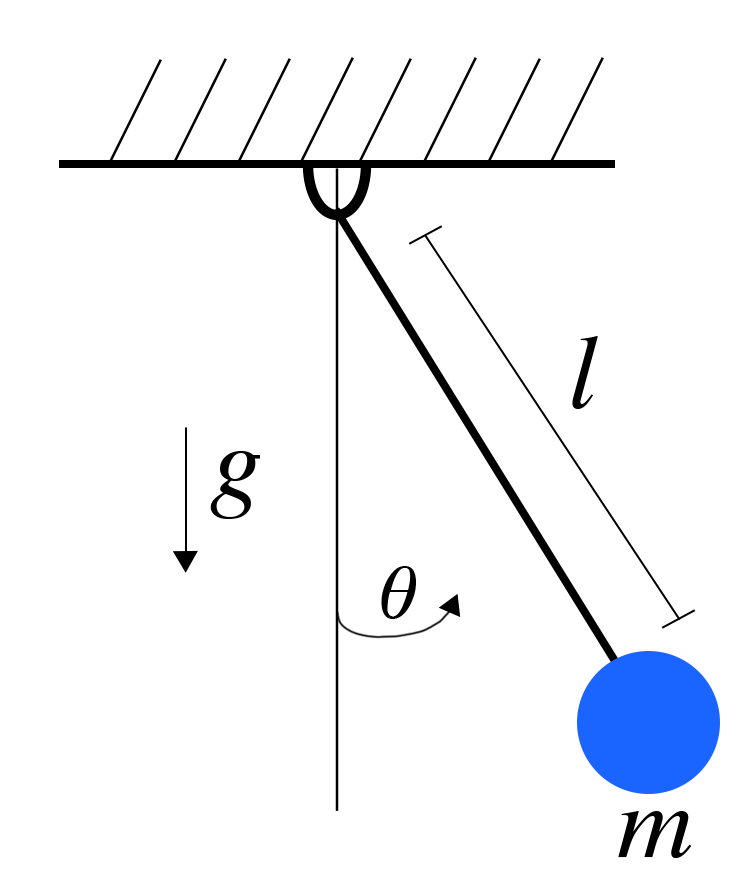
\includegraphics[width=0.3\linewidth]{figures/figure-pendulum.png}
    \captionof{figure}[Simple damped pendulum.]{Simple damped pendulum. In this figure $m$, $l$, and $\theta$ are the mass, length, and angle of the pendulum and $g$ and $b$ are the gravity constant and damping coefficient, respectively.} \label{fig:pendulum}
  \end{center}

  Let us investigate the stability of the pendulum found in figure \ref{fig:pendulum} above. The equations of motion of this simple damped pendulum are given by
  \begin{equation} \label{eq:pendulum}
    ml^2\ddot{\theta} + mgl\sin{\theta} = -b\dot{\theta},
  \end{equation}
  where $m$, $l$, and $\theta$ are the mass, length, and angle of the pendulum and $g$ and $b$\footnote{Some texts like \cite{khalilNonlinearControl2015} use $kl^2$ instead of $b$, where $k$ is the friction coefficient.} are the gravity constant and damping coefficient, respectively. Although a closed-form solution exists for this relatively simple example, it consists of integrating several elliptical integrals and provides us with relatively little intuition. More importantly, a closed-form solution is not guaranteed to exist for a more complicated system. However, from experience, we know that this damped pendulum (with $b > 0$) when released at an angle $\theta_{t_0}$ will lose energy due to air friction and, after some oscillations, will eventually rest at the lowest point, with minimal energy (i.e., $\theta = 2\pi k$). We can use this intuition to prove the stability of the system by looking at its total energy (kinetic + potential), which can be written down as
  \begin{equation}
    E\left(\theta, \dot{\theta}\right) = \frac{1}{2}ml^2\dot{\theta}^2 - mgl\cos{\theta}.
  \end{equation}
  Evaluating the time derivative of this energy function gives us
  \begin{equation}
    \frac{d}{dt}E = ml^2\dot{\theta}\ddot{\theta} + \dot{\theta}mgl\sin{\theta},
  \end{equation}
  and substituting in the system dynamics from equation \eqref{eq:pendulum} reveals
  \begin{equation}
    \frac{d}{dt}E = -b\dot{\theta} \le 0.
  \end{equation}
  Since this condition ensures that the system's energy will never increase, it is sufficient for proving stability. Unfortunately, since $\theta = 2\pi k$ is not the only minimum for which $\dot{E} = 0$, it does not prove that the system will converge to this minimum. It is also zero when the pendulum changes direction during the oscillating behaviour. As shown later, we can use \hyperref[th:lasalles]{La Salle's Invariance principle} to prove convergence.
\end{example}

The example above showed that a relatively simple energy function (i.e., mechanical energy) could be used to say something about the system stability without computing the complex analytical closed-form solution. Lyapunov's direct method generalizes this idea to systems that might not be stable in mechanical energy. It states that a general (non-)linear system is stable if a \textbf{positive definite} (energy) function $V\left(x\right)$, called a \textbf{Lyapunov function}, exists that decreases with time, meaning $\dot{V}\left(x\right)$ is \textbf{negative (semi-)definite}. These Lyapunov functions, when found, can be used to demonstrate several notions of stability when certain conditions are met. The Lyapunov conditions for the earlier defined stability notions (i.e., SISL, AS, EX) are shown without proof\footnote{The proofs can be found in chapter 4 of \cite{khalilNonlinearSystems2002} and section 3.3 of \cite{khalilNonlinearControl2015}.} in theorem \ref{th:auto_lyapunov_conditions}. In this theorem, the origin (i.e., $x = 0$) is taken as the equilibrium point. However, since any point can be shifted to the origin using a change of variables, it does not lead to a loss of generality.

%% Theorem - Lyapunov stability conditions for autonomous systems.
\begin{theorem}[list text=Sufficient conditions for stability of autonomous systems,after pre=\footnotetext{Theorem 4.1 and 4.10 of \cite{khalilNonlinearSystems2002} and theorem 3.3 \cite{khalilNonlinearControl2015} were slightly adjusted and combined to improve clarity.}]{Sufficient conditions for stability of autonomous systems \cite{khalilNonlinearSystems2002}\footnotemark}{auto_lyapunov_conditions}
  Let $x = 0$ be an equilibrium point of \eqref{eq:auto_nonlinear_system} and $D \subset\mathbb{R}^n$ be a domain containing $x = 0$. Let $V: D \rightarrow \mathbb{R}$ be a continuously differentiable function such that
  \begin{equation} \label{eq:lyapunov_psd_condition}
    V \left( 0 \right) = 0 \quad \textrm{and} \quad V \left( x \right)> 0 \quad \textrm{in} \quad D -\left\{ 0 \right\}
  \end{equation}
  \begin{equation}
    \dot{ V }\left( x \right) = \frac{\partial V}{\partial x} f \left( x \right)\le 0 \quad \textrm{in} \quad D
  \end{equation}
  then, $x = 0$ is (locally) \textbf{SISL}. Moreover, if
  \begin{equation} \label{eq:lyapunov_AS_condition}
    \dot{ V }\left( x \right) = \frac{\partial V}{\partial x} f \left( x \right)< 0 \quad \textrm{in} \quad D - \left\{ 0 \right\}
  \end{equation}
  then $x = 0$ is (locally) \textbf{AS}. Furthermore, if we have
  \begin{equation} \label{eq:lyapunov_ES_condition}
    \dot{ V }\left( x \right) = \frac{\partial V}{\partial x} f \left( x \right)\le- \alpha V \left( x \right) \quad \textrm{in} \quad D - \left\{ 0 \right\}
  \end{equation}
  then $x = 0$ is (locally) \textbf{ES}. Finally, if $D = R^n$, and \eqref{eq:lyapunov_psd_condition} holds for all $x \neq 0$, and $x$ is
  \begin{equation}
    \left\| x \right\| \rightarrow \infty \Rightarrow V\left(x\right) \rightarrow \infty
  \end{equation}
  then $x$ is said to be \textbf{radially unbounded}, meaning that trajectories cannot diverge to infinity even as $V$ decreases. Consequently, $x = 0$ is \textbf{GAS} if \eqref{eq:lyapunov_AS_condition} holds and \textbf{GES} if \eqref{eq:lyapunov_ES_condition} holds.
\end{theorem}

Please be aware that the conditions of theorem \ref{th:auto_lyapunov_conditions} used in Lyapunov's direct method are \textbf{sufficient conditions} for stability. Sufficient in that they only prove stability if a Lyapunov function $V$ is found. If they are violated for a given Lyapunov candidate, this does not prove that the equilibrium is unstable but simply that it is not a proper Lyapunov function. Lyapunov s theory contains several other theorems that can be used to prove the instability of an equilibrium point \cite{khalilNonlinearSystems2002}.

As shown in the pendulum example, for some systems, the derivative of the Lyapunov function $\dot{V}\left(x \right)$ ends up being \textbf{negative semi-definite}. As a result, for these systems, we can only prove SISL. However, it turns out that we can still show that an equilibrium point or set of equilibrium points is AS in some cases. For the damped pendulum, we, again from experience, know that for all the other points for which $\dot{E} = 0$ the system will not stay there because $\ddot{ \theta }\neq 0$. Consequently, the system will eventually converge to $\theta = 2 \pi k$, making it a stable equilibrium point. In mathematical terms, it means that $\theta = 2 \pi k$ is the largest positively invariant set and that, as $t \rightarrow\infty$, the system will eventually come to rest at this set. This relationship, called \textbf{\hyperref[th:lasalles]{LaSalle's invariance principle}}, is mathematically expressed in theorem \ref{th:lasalles}.

%% Theorem - LaSalle's invariance principle.
% NOTE: This theorem combines \cite{khalilNonlinearSystems2002} and https://underactuated.mit.edu/lyapunov.html.
\begin{theorem}[list text=LaSalle's invariance principle,after pre=\footnotetext{Theorem 4.4 of \cite{khalilNonlinearSystems2002} was reworded to improve readability.}]{LaSalle's invariance principle \cite{khalilNonlinearSystems2002}\footnotemark}{lasalles}
  Given \eqref{eq:auto_nonlinear_system} with $f$ being continuous. If a scalar function $V \left( x \right)$ exists with a continuous derivative such that
  \begin{equation}
    V \left( x \right)> 0, \quad \dot{ V }\left( x \right) \le 0
  \end{equation}
  and $V \left( x \right)\rightarrow\infty$ as $x \rightarrow \infty$, then $x$ will converge to the largest invariant set where $\dot{V}\left( x \right) = 0$.
\end{theorem}

As seen above, Lyapunov's direct method allows us to conclude the stability of (non-)linear systems when a valid Lyapunov function is found. From this, we can directly see the main weakness of this method, namely that finding these functions is not trivial. Since no general method exists for finding these Lyapunov functions in nonlinear systems, they must be found by trial and error. In practice, however, the situation is not as bad as it seems due to the tremendous amount of research on this topic. As a result, when trying to find a Lyapunov function for a new system, Lyapunov functions of prior research that consider similar systems can be used as candidates \cite{haddadNonlinearDynamicalSystems2011}. Moreover, in recent years several optimisation methods have been designed for specific types of systems that can iteratively find Lyapunov functions \cite{khalilNonlinearSystems2002,gieslReviewComputationalMethods2015,ravanbakhshLearningControlLyapunov2019}.

\subsection{Stability of unforced non-autonomous systems}
% NOTE: The equations in this section come from section 4.5 and 4.9 of \cite{khalilNonlinearSystems2002}.

In the previous section, we considered autonomous time-invariant systems. Doing this provided us with a good intuition of the workings of Lyapunov's direct method. In these systems, the solutions and thus the trajectories are dependent only on $\left(t - t _ 0\right)$. A specific initial condition $x\left(t_0\right)$ will therefore invariably lead to the same trajectory independent of the starting time $t_0$. Because of this, a system is always stable when a circle $\delta$ exists, for which all trajectories starting there will stay inside circle $\epsilon$. In most applications, however, the system solutions may depend on both $t$ and $t_0$. As a result, the circle $\delta$ is now not only dependent on $\epsilon$ but also on $t_0$. Because of this, there is no guarantee that a $\delta$ exists, dependent only on $\epsilon$, that is valid for all $t_0$. Therefore, the stability notions defined for autonomous systems no longer hold and must be extended such that they hold \textbf{uniformly} over time (i.e., holds for all $t_0$). For this purpose, let us consider the following \textbf{forced} non-autonomous system:
\begin{equation} \label{eq:unforced_nonlinear_system}
  \dot{ x }= f \left(t, x, u \right).
\end{equation}
In this $f : \left[0, \infty\right) \times \mathbb{R}^m \times \mathbb{R}^n \rightarrow \mathbb{R}^n$ is piecewise continuous in $t$ and locally Lipschitz in $x$ and $u$ on $\left[0 ,\infty\right)\times D$, and $D \subset \mathbb{R}^n$ is a domain that contains the origin $x = 0$. Further, let us assume for now that the system is \textbf{unforced} and thus does not have additional inputs other than time (i.e., $u=0$). For the origin of this system, $x=0$ to be \textbf{uniformly SISL}, for each $\epsilon > 0$, and any $t_0 \geq 0$, there must be a $\delta = \delta \left( \epsilon, t _ 0 \right)> 0$, dependent on initial time $t_0$, such that
\begin{equation}
  \left\| x\left(t_0\right)\right\| < \delta \Rightarrow \left\| x \left( t \right)\right\| < \epsilon, \quad \forall \; t\geq t_0.
\end{equation}
Extending this definition to the earlier mentioned stability notions results in definition \ref{def:unforced_nonauto_lyapunov_stabiliy}.
%% Definition - Time-dependent stability notions.
\begin{definition}[list text=Time-dependent stability notions,after pre=\footnotetext{Definition 4.2 of \cite{khalilNonlinearControl2015} was slightly changed for consistency with earlier stability notions.}]{Time-dependent stability notions \cite{khalilNonlinearControl2015}\footnotemark}{unforced_nonauto_lyapunov_stabiliy}
  The equilibrium point $x = 0$ of the \textbf{unforced} (i.e., $u=0$) system given in \eqref{eq:unforced_nonlinear_system} is
  \begin{enumerate}
    \item \textbf{Uniformly SISL}, if there exists a class $\mathcal{K}$ function $\alpha$ and a positive constant $c$, independent of $t_o$, such that
          \begin{equation}
            \left\|x\left(t\right)\right\| < \alpha \left( \left\|x \left( t_0 \right) \right\|\right), \quad \forall \; t \geq t_0 \geq 0, \quad \forall \; \left\|x\left(t_0 \right) \right\| < c.
          \end{equation}
    \item \textbf{Uniformly AS} if there exists a class $\mathcal{KL}$ function $\beta$ and a positive constant $c$, independent of $t_0$, such that
          \begin{equation}
            \left\|x\left(t\right)\right\| < \beta \left( \left\|x \left( t_0 \right) \right\|, t-t_0\right), \quad \forall \; t \geq t_0 \geq 0, \quad \forall \; \left\|x\left(t_0 \right) \right\| < c.
          \end{equation}
    \item	\textbf{Globally uniformly AS} if the previous inequality holds $\forall \; x \left( t _ 0 \right)$.
    \item	\textbf{Uniformly ES} if there exist positive constants $c$, $M$, and $\lambda$ such that
          \begin{equation}
            \left\|x\left(t \right) \right\| \leq Me^{-\lambda\left(t-t_0\right)} \cdot \left\|x\left(t_0 \right) \right\|, \quad \forall \; \left\|x\left(t_0 \right) \right\| < c.
          \end{equation}
    \item \textbf{Globally uniformly ES} if the previous inequality holds $\forall \; x \left( t _ 0 \right)$.
  \end{enumerate}
\end{definition}
In these notions, so-called class $\mathcal{K}$ and class $\mathcal{KL}$ functions (see definition \ref{def:k_kl_functions}) were used for transparency \cite{khalilNonlinearSystems2002}. These functions are used to generalise $\epsilon$ of the previous stability notions while $c$ can be seen as a generalization of $\delta$.

%% Definition - K and KL functions.
\begin{definition}[list text=Class $\mathcal{K}$ and class $\mathcal{KL}$ functions]{Class $\mathcal{K}$ and class $\mathcal{KL}$ functions \cite{khalilNonlinearControl2015}}{k_kl_functions}
  \begin{enumerate}
    \item A scalar continuous function $\alpha \left( r \right)$, defined for $r \in\left[0, a \right)$, belongs to class $\mathcal{K}$ if it is strictly increasing and function $\alpha \left( 0 \right)\equiv 0$. It belongs to class $\mathcal{K}_\infty$ if it is defined for all $r \geq 0$ and $\alpha \left( r \right)\rightarrow\infty$ as $r \rightarrow\infty$.
    \item A scalar continuous function $\beta \left( r, s \right)$, defined for $r \in\left[0, a \right)$, and $s \in\left[0, \infty\right)$, belongs to class $\mathcal{KL}$ if, for each fixed $s$, the mapping $\beta \left( r, s \right)$ belongs to class $\mathcal{K}$ with respect to $r$ and, for each fixed $r$, the mapping $\beta \left( r, s \right)$ is decreasing with respect to $s$ and $\beta \left( r, s \right)\rightarrow 0$ as $s \rightarrow\infty$.
  \end{enumerate}
\end{definition}

Now that we have defined the stability notions for unforced non-autonomous systems, we can determine the accompanying Lyapunov stability conditions. These Lyapunov stability conditions are presented without proof\footnote{The proofs can be found in section 4.5 of \cite{khalilNonlinearSystems2002}.} in theorem \ref{th:unforced_auto_lyapunov_conditions} below. The big difference with theorem \ref{th:auto_lyapunov_conditions} is that now $f$ and $V$ are dependent on time. Consequently, these conditions now also contain time derivates and several time-independent bounds (i.e., $W_1$, $W_2$, $W_3$, $k_{\left\{n \; \in \; \mathbb{R}: \; 1 - 3 \right\}} \left\|x^a\right\|$).

%% Theorem - Lyapunov stability conditions for unforced non-autonomous systems.
\begin{theorem}[list text=Sufficient conditions for stability of unforced non-autonomous systems,after pre=\footnotetext{This theorem combines theorem 4.1-4.3 of \cite{khalilNonlinearControl2015}. These theorems were slightly adjusted for clarity.}]{Sufficient conditions for stability of unforced non-autonomous systems \cite{khalilNonlinearControl2015}\footnotemark}{unforced_auto_lyapunov_conditions}
  \underline{Uniformly SISL}

  Let the origin $x = 0$ be an equilibrium point of the \textbf{unforced} (i.e., $u=0$) system \eqref{eq:unforced_nonlinear_system} and $D \subset\mathbb{R}^n$ be a domain containing $x = 0$. Suppose \eqref{eq:unforced_nonlinear_system} is piecewise continuous in $t$ and locally Lipschitz in $x$ for all $t \geq 0$ and $x \in D$. Let $V \left(t, x \right)$ be a continuously differentiable function such that
  \begin{equation} \label{eq:uniformly_sisl_psd}
    W_1\left(x \right)\leq V\left(t, x\right) \leq W_2\left(x \right)
  \end{equation}
  \begin{equation} \label{eq:uniformly_sisl}
    \frac{\partial V}{\partial t} + \frac{\partial V}{\partial x} f \left( t, x \right) \le 0
  \end{equation}
  for all $t \geq 0$ and $x \in D$, where $W_1\left( x \right)$ and $W_2\left( x \right)$ are continuous positive definite class $\mathcal{K}$ functions on $D$. Then the origin is \textbf{uniformly SISL}.
  \vspace{1em}

  \underline{(Globally) Uniformly AS}

  Suppose the assumptions above for uniformly SISL are satisfied with inequality \eqref{eq:uniformly_sisl} strengthened to
  \begin{equation} \label{eq:uniformly_AS}
    \frac{\partial V}{\partial t}+\frac{\partial V}{\partial x} f \left( t, x \right)\le W_3\left(x \right)
  \end{equation}
  for all $t \geq 0$ and $x \in D$, where $W_3\left( x \right)$ is a continuous positive definite function on $D$. Then, the origin is \textbf{uniformly AS}. Moreover, if some constants $r$ and $c$ are chosen such that $B_r = \left\{ \left\|x\right\| \leq r \right\} \subset D$ and $c < \min_{\left\|x\right\|=r}W_1\left(x\right)$, then every trajectory starting in $\left\{ x \in B_r\; |\; W_2\left(x\right) \le c \right\}$ satisfies
  \begin{equation}
    \left\|x\left(t \right) \right\| \leq \beta\left(\left\|x\left(t_0 \right)\right\|, t-t_0\right), \quad \forall \; t \ge t_0 \ge 0
  \end{equation}
  for some class $\mathcal{KL}$ function $\beta$. Finally, if $D = \mathbb{R}^n$ and $W_1 \left( x \right)$ is radially unbounded, then the origin is \textbf{globally uniformly AS}.
  \vspace{1em}

  \underline{(Globally) Uniformly ES}

  Suppose the assumptions above for uniformly SISL are satisfied with inequality \eqref{eq:uniformly_sisl_psd} and \eqref{eq:uniformly_sisl} strengthened to
  \begin{equation}
    k_1\left\|x\right\|^a \leq V\left(t, x\right) \leq k_2 \left\|x\right\|^a
  \end{equation}
  \begin{equation}
    \frac{\partial V}{\partial t}+\frac{\partial V}{\partial x} f \left( t, x \right)\le - k_3 \left\|x\right\|^a
  \end{equation}
  for all $t \geq 0$ and $x \in D$, where $k_1$, $k_2$, $k_3$ and $a$ are positive constants. Then the origin is \textbf{ES}. If the assumptions hold globally, the origin will be \textbf{globally ES}.
\end{theorem}

Similar to the autonomous case, there are situations where the Lyapunov analysis can only prove uniform SISL because $W_3 \left( x \right)$ ends up being positive semi-definite. In these cases, an extension of \hyperref[th:lasalles]{LaSalle's invariant principle} for non-autonomous systems, called \textbf{Barbalat's lemma}, can be used to prove AS \cite{khalilNonlinearSystems2002}.

\subsubsection{Boundedness and ultimate boundedness}
% NOTE: Theory for this section can be found in \cite{khalilNonlinearControl2015} section 4.3.

In the previous sections, the nonlinear systems \eqref{eq:auto_nonlinear_system} and \eqref{eq:unforced_nonlinear_system} were assumed to have distinct equilibrium points. However, Lyapunov's stability theory can also show the \textbf{boundedness} of the nonlinear system solution when there is no equilibrium point at the origin. Let us, for example, consider a simple nonlinear system in which the following scalar equation governs the system behaviour:
\begin{equation}
  \dot{ x }=- x + \delta \sin{\left( t \right)}, \quad x \left(t_0\right)= a, \quad a > \delta > 0.
\end{equation}
The solution to this system can be expressed as
\begin{equation}
  x \left( t \right) = e^{-\left(t-t_0\right)} a + \delta \int_{t_0}^{t}e^{-\left( t - \tau \right)} \sin{\tau} d\tau.
\end{equation}
This system has no clear equilibrium point due to the presence of the trigonometric term $\boldsymbol{\sin{t}}$. It, however, is not unstable since it satisfies the following bound:
\begin{equation}
  \left| x \left( t \right)\right| \le e^{-\left( t -t_0\right)} a + \delta \int_{t_0}^{ t }e^{-\left( t - \tau \right)} d\tau = e^{-\left(t -t_0 \right)}a + \delta \left[ 1 -e^{-\left( t -t_0\right)} \right] \le a,
  \quad \forall \; t \ge t_0.
\end{equation}
As a result, the system is shown to be \textbf{uniformly bounded (UB)} by $a$ for all $t \geq t_0$, that is, with a bound independent of $t_0$. Although this bound is valid for all times $t \geq t_0$, since it does not consider the exponentially decaying term, it becomes a conservative estimate of the solution as time progresses. We can, therefore, instead pick any number $b$, such that $\delta < b < a$, to get the following bound:
\begin{equation}
  \left| x \left( t \right)\right|\le b ,\quad \forall \; t \geq t_0 + ln {\left(\frac{ a - \delta }{ b - \delta }\right)}= t_o + T.
\end{equation}
This new bound $b$, which is again independent of $t_0$, provides us with a less conservative estimate of the solution after a transient period $T$ has passed (see figure \ref{fig:boundedness_2D}). In this case, the system is said to be uniformly \textbf{ultimately bounded (UUB)}, with bound $b$ being the ultimate bound. These notions are summarized in definition \ref{def:boundedness} below. For autonomous systems, the prefix "uniformly" can be dropped since it only depends on $t-t_0$.

%% Figure - Boundedness.
\begin{figure}
  \centering
  \begin{subfigure}[c]{0.55\textwidth}
    \centering
    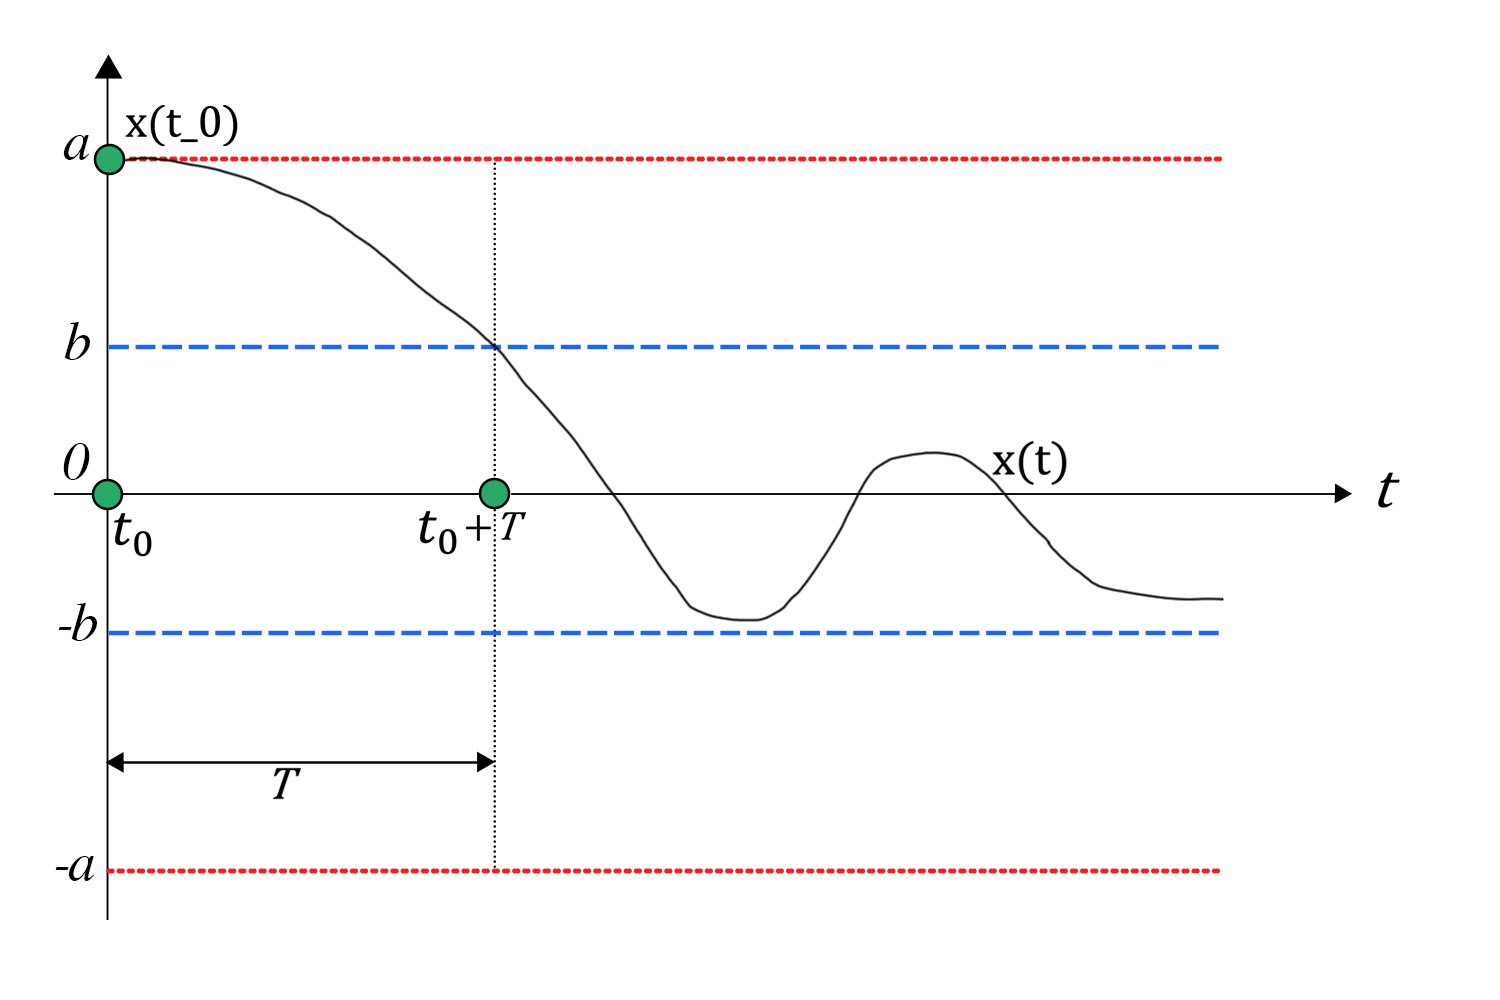
\includegraphics[width=\linewidth]{figures/figure-bounce.jpg}
    \caption{} \label{fig:boundedness_2D}
  \end{subfigure}
  \hspace{4mm}
  \begin{subfigure}[c]{0.31\textwidth}
    \centering
    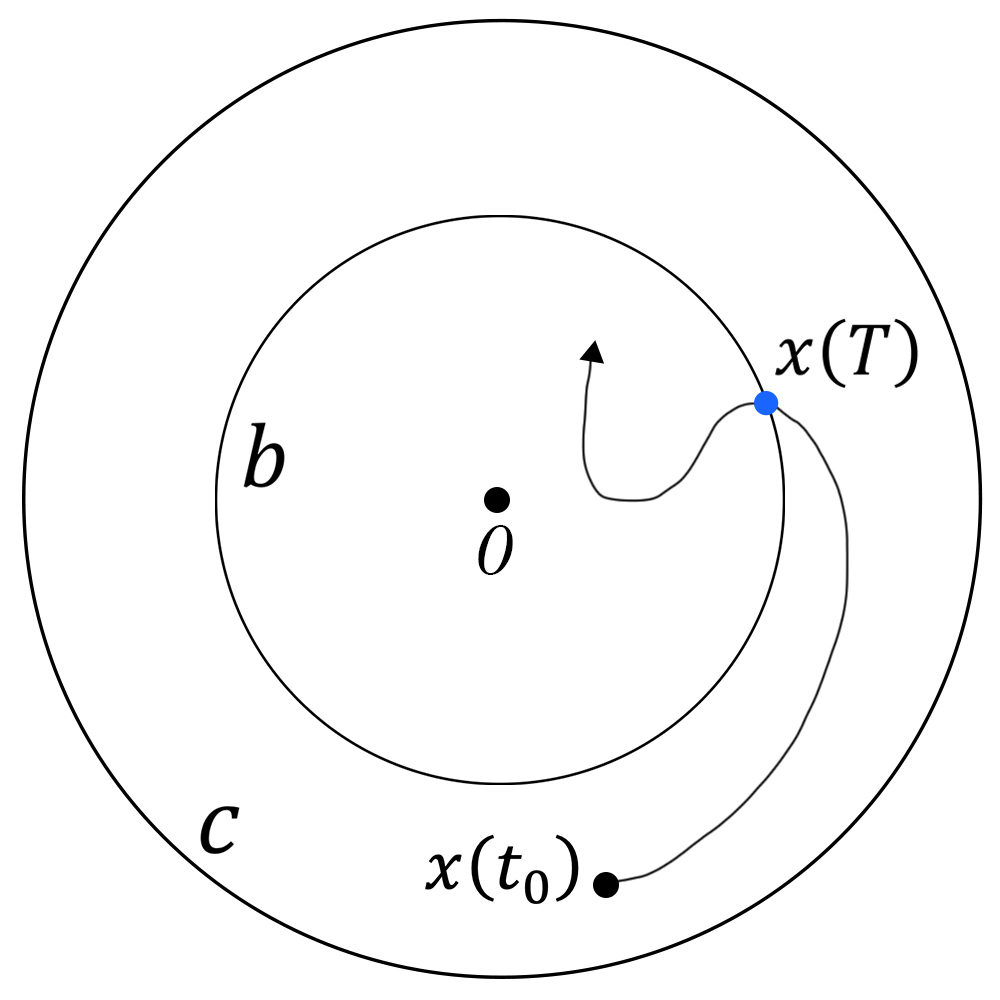
\includegraphics[width=\linewidth]{figures/figure-uub.jpg}
    \caption{} \label{fig:boundedness_3D}
  \end{subfigure}%

  \caption[Visualization of uniform and ultimate boundedness.]{Uniform and ultimate boundedness visualized in 1D (figure \ref{fig:boundedness_2D}) and 2D (figure \ref{fig:boundedness_3D}). In these figures, $t_0$ is the initial time, $T$ the time after the transient period, $x$ the trajectory and $a$ and $b$ are the uniform and ultimate bound, respectively.} \label{fig:boundedness_notions}
\end{figure}

%% Definition - Uniform and ultimate boundedness.
\begin{definition}[list text=Uniform and ultimate boundedness]{Uniform and ultimate boundedness \cite{khalilNonlinearControl2015}}{boundedness}
  The solutions of the \textbf{unforced} (i.e., $u=0$) system \eqref{eq:unforced_nonlinear_system} are
  \begin{itemize}
    \item \textbf{UB} if there	exists $c > 0$, independent of $t_0$, and for every $a \in\left( 0, c \right)$, there is $\beta > 0$, dependent on $a$ but independent of $t_0$, such that
          \begin{equation} \label{eq:uniform_boundedness}
            \left\|x\left(t_0\right)\right\| \le a \Rightarrow \left\|x\left(t \right)\right\| \le \beta, \quad \forall \; t \ge t_0.
          \end{equation}
    \item \textbf{Globally UB} if \eqref{eq:uniform_boundedness} holds for arbitrarily large $a$.
    \item	\textbf{UUB} with ultimate bound $b$ if there exists a positive constant $c$, independent of $t_0$, and for every $a \in\left( 0, c \right)$, there is a $T \geq 0$, dependent on $a$ and $b$ but independent of $t_0$, such that
          \begin{equation} \label{eq:uniform_ultimately_boundedness}
            \left\|x\left(t_0\right)\right\| \le a \Rightarrow \left\|x\left(t \right)\right\| \le b, \quad \forall \; t \ge t_0 + T.
          \end{equation}
    \item \textbf{Globally UUB} if \eqref{eq:uniform_ultimately_boundedness} holds for arbitrarily large $a$.
  \end{itemize}
\end{definition}

It is important to note that in contrast to $\epsilon$ in SISL, here, the (ultimate) bound $b$ can not be made arbitrarily small by starting closer to the equilibrium point of origin. This bound instead depends on the system dynamics, uncertainties and disturbances. As a result, these stability notions can be seen as "milder" forms of SISL. As they are not defined around specific equilibrium points, they only require that trajectories converge to a given bound in finite time and stay therein for all future times (see figure \ref{fig:boundedness_3D}). Therefore, they are easier to achieve in practical dynamical systems subject to uncertainties and disturbances.

Like the other stability notions, a Lyapunov analysis can be used to investigate the UB and UUB of nonlinear systems. Since the Lyapunov conditions used in this analysis are very similar to those in theorem \ref{th:unforced_auto_lyapunov_conditions}, they will not be displayed here. Instead, they can be found in \cite{khalilNonlinearControl2015} with their proof and several examples.

\subsubsection{Stability of perturbed systems}
% NOTE: Theory for this section can be found in \cite{khalilNonlinearSystems2002} section 9.1.

Besides being time-dependent and possibly lacking distinct equilibrium points, real systems can also be subject to perturbations caused by modelling errors, ageing, uncertainties, and disturbances. It turns out that for stable unperturbed systems, Lyapunov's stability theory can be extended to include perturbations when information about these perturbations, like an upper bound, is available. To demonstrate this, let us extend the system of \eqref{eq:unforced_nonlinear_system} with a perturbation $g\left(t, x\right)$:
\begin{equation} \label{eq:perturbed_nonlinear_system}
  \dot{ x }= f \left(x, t, u\right)+ g \left(t, x\right), \quad u = 0.
\end{equation}
Like $f$, $g :\left[0, \infty\right)\times D \rightarrow\mathbb{R}^n$ is also piecewise continuous in $t$ and locally Lipschitz in $x$ and $u$. Further $g$ can be a vanishing (i.e., $g \left( t, 0 \right)= 0$) or non-vanishing (i.e., $g \left(t, 0 \right)\neq 0$). Now suppose that the nominal system \eqref{eq:unforced_nonlinear_system} has an ES equilibrium point $x = 0$, and $V\left(t, x \right)$ is a Lyapunov function that satisfies
\begin{equation}
  c_1 \left\|x\right\|^2 \le V\left(t, x \right) \le c_2 \left\|x \right\|^2,
\end{equation}
\begin{equation} \label{eq:perturbed_lyapunov_condition2}
  \frac{\partial V}{\partial t} + \frac{\partial V}{\partial x}{f \left( t, x \right)} \le - k_3 \left\|x\right\|^2,
\end{equation}
\begin{equation} \label{eq:perturbed_lyapunov_condition3}
  \left\|\frac{\partial V}{\partial x}\right\| \le c_4 \left\|x\right\|,
\end{equation}
for all $\left( t, x \right) \in \left[0, \infty\right) \times D$ for some positive constants $c_1$, $c_2$, $c_3$ and $c_4$. These conditions, which can be seen as the inverse or converse\footnote{More information on the inverse Lyapunov theorems can be found in section 4.7 of \cite{khalilNonlinearSystems2002}.} of the Lyapunov conditions in theorem \ref{th:unforced_auto_lyapunov_conditions}, prove that some $V\left(t, x\right)$ exists, given an ES equilibrium exists.

Now let us assume that we know $g$ is a vanishing perturbation (i.e., $g \left( t, 0 \right)= 0$) which is linearly bounded by
\begin{equation} \label{eq:perturbation}
  \left\|g\left( t, 0 \right)\right\| \le \gamma \left\|x\right\|, \quad \forall \; t \ge 0, \quad \forall \; x \in D,
\end{equation}
in which $\gamma$ is a nonnegative constant. Given this information and the fact that the nominal system has an ES equilibrium point, a natural approach would be to use the Lyapunov function of the nominal system as a candidate for investigating the stability of the perturbed system. Doing this results in the following derivative of $V$ along the trajectories of \eqref{eq:perturbed_nonlinear_system}:
\begin{equation} \label{eq:perturbed_auto_lyap_derivative}
  \dot{ V }\left( t, x \right)=\frac{\partial V}{\partial t} + \frac{\partial V}{\partial x} f \left( t, x \right) + \frac{\partial V}{\partial x} g \left(t, x \right).
\end{equation}
The first two terms on the right-hand side of \eqref{eq:perturbed_auto_lyap_derivative} represent the contribution of the nominal system. Because these terms are always negative definite, the resulting $\dot{V}\left( t, x\right)$ is also negative definite, and condition \eqref{eq:perturbed_lyapunov_condition2} is satisfied. The third term, $\left[\frac{\partial V}{\partial x}\right] g \left(t, x \right)$, represents the effect of the perturbation. Since no exact knowledge is available about $g$ the effect of this term on the definiteness of $\dot{ V }\left( t, x \right)$ is unknown. Therefore, we can at best use the linear bound on $g$, which was given in \eqref{eq:perturbation}, to investigate the worst-case scenario. Using this information with \eqref{eq:perturbed_lyapunov_condition2} and \eqref{eq:perturbed_lyapunov_condition3} results in the following inequality:
\begin{equation}
  \dot{ V }\left( t, x \right) \le - c_3\left\|x\right\|^2 + \left\|\frac{\partial V}{\partial x}\right\|\left\|g\left(t, x\right)\right\| \le -c_3\left\|x\right\|^2+c_4\left\|x\right\|^2.
\end{equation}
From this, we can determine that if $\gamma$ is small enough to satisfy the bound
\begin{equation}
  \gamma<\frac{c_3}{c_4},
\end{equation}
then
\begin{equation}
  \dot{ V }\left( t, x \right) \le - \left( c_3 - \gamma c_4 \right) \|x\|^2, \quad \left(c_3 - \gamma c_4\right) > 0.
\end{equation}
Using Theorem~\ref{th:unforced_auto_lyapunov_conditions} it can therefore be concluded that the origin of the nominal system is also a (globally) ES equilibrium point of the perturbed system. As a result, although the perturbation can disturb the system trajectories away from the equilibrium point, the system will return to this equilibrium point when it is gone. A similar relationship can be derived when the nominal system has an AS equilibrium point \cite{khalilNonlinearControl2015}.

In the case that $g$ is a non-vanishing perturbation, the equilibrium point $x = 0$ of the nominal system \eqref{eq:unforced_nonlinear_system} may no longer be the equilibrium point of the perturbed system \eqref{eq:perturbed_nonlinear_system}. As a result, the reasoning above is no longer valid. For these systems, we can at best prove that $x\left(t\right)$ is bounded by a small bound (i.e., UUB), if the perturbation is relatively small. More information about this extension of UB and UUB to non-vanishing perturbed systems can be found in Chapter 9 of \cite{khalilNonlinearSystems2002}.

\subsection{Stability of forced non-autonomous systems}
% TODO: The lyapunov function that adheres for these forced non-autonomous systems is called a Lyapunov Control function.

The previous chapter extended Lyapunov's stability theory to work for unforced, non-autonomous and perturbed systems. In most cases, however, we are not interested in the stability of free or perturbed systems but that of the system when it is being controlled (i.e., $u \neq 0$). Two distinct approaches can be taken for investigating the stability of controlled systems: the state-space approach and the input-output approach. In the state-space approach, a detailed model of the inner structure of the system is used to investigate the behaviour of the state variables. On the other hand, the input-output approach treads the system as a black box and relates the system's output directly to the input. These two approaches seed two distinct stability notions: \textbf{input-to-state stability (ISS)} and \textbf{input-output stability (IOS)}. IOS is used for systems with no exact state model, for example, systems which can only be approximated due to time delays. Since a dynamics model is readily available for robot manipulators, the rest of the text will focus on ISS. However, concepts like dissipativity and passivity explained below can also be applied to IOS. Interested readers can check out \cite{khalilNonlinearControl2015} for more information.

\subsubsection{Input-to-state stability}
% NOTE: Theory for this section can be found in \cite{khalilNonlinearControl2015} section 4.4.

Roughly speaking, a system is said to be ISS if it is GAS or GES in the absence of external inputs and the trajectories $x \left( t \right)$ stay bounded for any bounded input $u \left( t \right)$. The mathematical definition naturally follows the previous sections on UB and perturbed systems if we consider the new input u as a bounded disturbance to the unforced system $\dot{ x }= f \left( x, t, 0 \right)$. For this perturbed system, since $u$ is bounded, it might be possible to show that $\dot{ V }$ is negative (semi-)definite outside a ball of radius $\mu$, where $\mu$ depends on the upper bound of $u$ (i.e., $\sup{\left\|u\right\|}$). As a result, we can use the concept of UB to arrive at the formal definition of ISS shown in definition \ref{def:input_to_state_stability}.

%% Definition - Input-state stability
\begin{definition}[list text=Input-to-state stability,after pre=\footnotetext{Definition 4.4 of \cite{khalilNonlinearControl2015} was slightly changed for consistency with the rest of the text.}]{Input-to-state stability \cite{khalilNonlinearControl2015}\footnotemark}{input_to_state_stability}
  The \textbf{forced} (i.e., $u \ge 0$) system \eqref{eq:unforced_nonlinear_system} is \textbf{input-to-state stable} if there exists a class $\mathcal{KL}$ function $\beta$ and a class $\mathcal{K}$ function $\gamma$ such that for any $t_0 \geq 0$, any initial state $x \left( t_0 \right)$, and any bounded input $u\left( t \right)$, the solution $x \left( t \right)$ exists for all $t \geq t_0$ and satisfies
  \begin{equation}
    \left\|x\left(t\right)\right\| \le \max \left\{ \beta\left(\left\|x\left(t_0 \right)\right\|, t-t_0\right), \ \gamma \left(\sup_{t_0 \leq \tau \leq t}{\left\|u\left(\tau \right)\right\|} \right)\right\}, \quad \forall \; t \geq t_0.
  \end{equation}
\end{definition}

Several Lyapunov-based approaches exist in the literature to prove the ISS of systems: dissipativity, robustness margins and classical Lyapunov-like conditions \cite{khalilNonlinearSystems2002,sontagInputtoStateStabilityProperty1995}. Of these approaches, the notion of dissipativity and its special case passivity is especially convenient when working with the interconnected systems often encountered in control.

\subsubsection{Contraction}
// TODO: quickly explain contraction.

\subsubsection{Passivity}
% NOTE: Theory for this section can be found in chapter 2 of \cite{baoProcessControlPassive2007} and chapter 3 of \cite{ebenbauerDissipationInequalitiesSystems2009}.

%% Figure - RLC circuit.
\begin{figure}
  \centering
  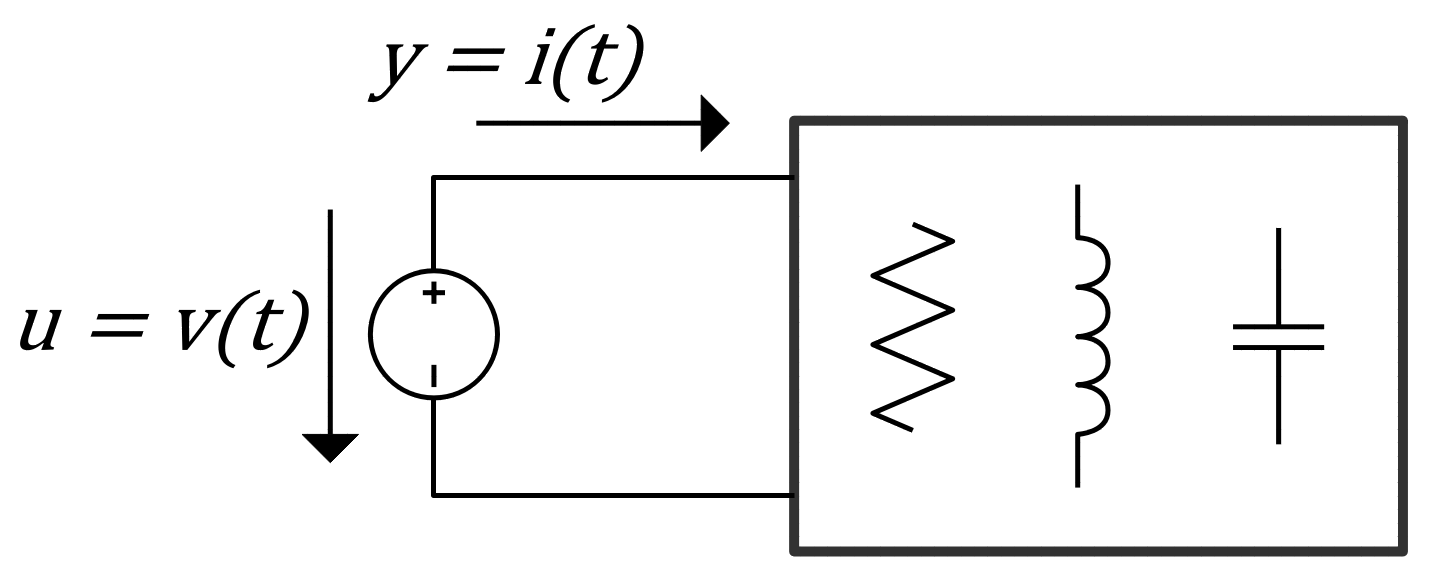
\includegraphics[width=0.55\linewidth]{figures/RLC_circuit.png}
  \caption[Schematic diagram of a general RLC circuit.]{Schematic diagram of a general RLC circuit containing a combination of (passive) resistances, inductors and capacitors. In this, $y$ and $x$ represent the input and output while $v$ and $i$ represent the voltage and current, respectively.} \label{fig:rlc_circuit}
\end{figure}

The concept of a passive system first emerged in the circuit theory field from the energy dissipation in passive component \cite{popovHyperstabilityControlSystems1973}. In electrical networks, an electronic component is called passive if it does not require electrical energy to operate. It can only receive energy from other components and either dissipate, absorb, or store it in an electric or magnetic field. Because of this, networks that only contain passive elements will not generate energy and are, therefore, stable \cite{andersonNetworkAnalysisSynthesis2013}. An example of such a passive network is the general RLC circuit depicted in figure \ref{fig:rlc_circuit}. Since it consists of only passive elements (e.g., inductors, resistors and capacitors), it cannot supply more energy to its environment than it receives. As the power supplied to this network equals the product of voltage and current (i.e., $p \left( t \right)= v \left( t \right) i \left( t \right)$) this results in the following inequality:
\begin{equation}
  E \left( t_1 \right)- E \left( t_0 \right)\le\int_{ t_0 }^{ t_1 } v \left( t \right) i \left( t \right)dt, \quad t_0 \le t_1.
\end{equation}
This inequality which relates the total energy stored in the network $E\left(t\right)$ to the energy supplied to the network, holds for all passive electrical systems.

This notion of passivity was later generalized to other dissipative systems through the introduction of a \textbf{storage function} (energy stored in the system) and a \textbf{supply rate} (externally supplied energy) \cite{willemsDissipativeDynamicalSystems1972a,willemsDissipativeDynamicalSystems1972}. A system is said to be dissipative if its energy (storage function) increases no more than the energy provided (via the supply rate) during a given time interval. This relationship is mathematically expressed in definition \ref{def:dissipativity} below.

%% Definition - Dissipativity.
\begin{definition}[list text=Dissipative system]{Dissipative system \cite{baoProcessControlPassive2007}}{dissipativity}
  System $H$ with \textbf{supply rate} $w \left( t \right)$ is said to be \textbf{dissipative} if there exists a nonnegative real function $S \left( x \right): X \rightarrow\mathbb{R}^+$ called the \textbf{storage function}, such that, for all $t_1 \geq t_0 \geq 0$, $x\left(t_0\right) \in X$ and $u \in U$,
  \begin{equation}
    S \left( x_1 \right)- S \left( x\left(t_0\right) \right) \le \int_{ t_0 }^{ t_1 } w \left( t \right) dt
  \end{equation}
  where $x_1 = \phi \left(t_1, t_0, x\left(t_0\right), u \right)$ and $\mathbb{R}^+$ is a set of nonnegative real numbers.
\end{definition}

In this definition, $H$ can be any general (non-)linear system, while the supply rate $w \left( t \right)$, which determines the type of dissipativity, can be any bounded function defined on the input and output space (i.e., $\int_{ t_0 }^{ t_1 } w \left( t \right)dt<\infty$). If the storage function S is continuously differentiable, this relationship simplifies to
\begin{equation}
  \frac{ dS \left( x \left( t \right)\right)}{ dt }\le w \left( t \right),
\end{equation}
which emphasizes the storage function's positive semi-definiteness. When a bilinear supply rate is used, we receive the general definition of a passive system given in definition \ref{def:passivity}. This definition spans a broad spectrum of passive systems, with \textbf{lossless} and \textbf{state strictly passive} systems being the most extreme cases. Where lossless systems store all energy supplied to them, strictly passive systems lose additional energy due to, for example, heat or friction.

%% Definition - Passivity.
\begin{definition}[list text=Passive system,after pre=\footnotetext{Definition 2.7 of \cite{baoProcessControlPassive2007} was combined with a slightly modified version of definition 5.3 of \cite{khalilNonlinearControl2015}.}]{Passive system \cite{khalilNonlinearControl2015, baoProcessControlPassive2007}\footnotemark}{passivity}
  A system is said to be \textbf{passive} if it is dissipative with respect to the following supply rate:
  \begin{equation}
    w \left(u \left(t\right), y \left( t \right)\right)={ u \left( t \right)}^T y \left( t \right)
  \end{equation}
  and the storage function $S \left( x \right)$ satisfies $S \left( 0 \right)= 0$. Moreover, it is
  \begin{enumerate}
    \item \textbf{Lossless} if $\dot{ S }={ u \left( t \right)}^T y \left( t \right)$.
    \item \textbf{Input strictly passive} if $\dot{S} + {u \left(t \right)}^T \varphi \left(u \left(t \right)\right) \le {u \left(t \right)}^T y \left(t \right) \ and \ {u \left( t \right)}^T \varphi \left(u \left( t \right)\right) > 0, \quad \forall \; u \neq 0$.
    \item \textbf{Output strictly passive} if $\dot{S} + {y \left(t \right)}^T \rho \left(y \left(t \right)\right) \le {u \left(t \right)}^T y \left(t \right) \ and \ {y \left( t \right)}^T \varphi \left(y \left(t \right)\right) > 0, \quad \forall \; u \neq 0$.
    \item \textbf{Strictly passive} if $\dot{S} + \psi \left(x \right) \le {u \left(t \right)}^T y \left(t \right)$ for some positive definite function $\psi$.
  \end{enumerate}
  In all cases, the inequality should hold for all $\left(x, u\right)$. A system that does not adhere to these conditions is said to be \textbf{active}.
\end{definition}

From the definitions above, it is easy to see that the inequality reduces to the aforementioned Lyapunov inequality $\dot{ V }\left( x \left( t \right)\right)\le 0$ when $u = 0$. Because of this, Lyapunov functions can be used as candidate energy functions in dissipative and passive systems. To better understand the relationship between passivity and stability, let us apply the concept of passivity to the earlier used simple damped pendulum (see example \ref{ex:passivity}).

%% EXAMPLE - Passivity.
% NOTE: Example was based on example 5.5 of \cite{khalilNonlinearControl2015}.
\begin{example}{Passivity analysis of simple damped pendulum}{passivity}
  Consider the simple damped pendulum of example \ref{ex:pendulum}. Let us add an input torque $u$ and rewrite the equations of motion in \eqref{eq:pendulum} as two coupled first-order differential equations:
  \begin{equation} \label{eq:pendulum_state_form}
    \dot{x}_1 = \dot{x}_2, \quad \dot{x}_2 = -\frac{g}{l} \sin(x_1) - \frac{b}{ml^2}x_2 + \frac{1}{ml^2}u,
  \end{equation}
  where $x_1$ is the pendulum angle $\theta$. Now let us take $y = x_2$ as the output and use the expression for the total energy we found in example \ref{ex:pendulum} as a candidate energy function $S$:
  \begin{equation}
    S \left(x_1, x_2 \right) = \frac{1}{2} m l^2 x_2^2 - mgl \cos{x_1}.
  \end{equation}
  Note that this function is positive definite but not positive semi-definite since it is zero at points other than the origin. Evaluating the time derivative of this energy function gives us
  \begin{equation}
    \dot{S}\left(x_1, x_2\right) = ml x_2 \left( l \dot{x}_2 + g \sin{x_1}\right),
  \end{equation}
  and substituting in the system dynamics from equation \eqref{eq:pendulum_state_form} reveals
  \begin{equation}
    \dot{S}\left(x_1, x_2 \right) = -b x_2 + x_2 u.
  \end{equation}
  Using the passivity relationship in definition \ref{def:passivity} and definition \ref{def:dissipativity} results in the following inequality:
  \begin{equation}
    \dot{S} - u^T y = -b x_2 + x_2 u - u x_2 = -b x_ 2^2 \le x_2 u - u x_2 \le 0.
  \end{equation}
  Hence, the pendulum is \textbf{passive} when $b = 0$ and is \textbf{strictly (output) passive} when $b > 0$.
\end{example}

The pendulum example above showed that the concept of passivity implies stability if a positive definite storage function is used. However, because the storage function in \ref{def:dissipativity} is only required to be positive semi-definite (i.e., nonnegative), stability is not always guaranteed by passivity. This is because the presence of an unobservable unstable part of the system still has the potential to destabilise the equilibrium $x=0$. To exclude these situations, additional conditions like zero-state detectability and observability are required:

%% Definition - Zero-state detectability and observability.
\begin{definition}[list text=Zero-state detectability and observability]{Zero-state detectability and observability \cite{baoProcessControlPassive2007}}{zero_state}
  A system H is \textbf{zero-state observable (ZSO)} if for any $x \in X$,
  \begin{equation} \label{eq:zero_state_observable}
    y\left(t\right) = h\left(\phi\left(t, t_0, x, u \right)\right) = 0, \quad u = 0, \quad \forall \; t \geq t_0 \geq 0 \quad implies \ x = 0,
  \end{equation}
  and the system is \textbf{locally ZSO} if there exists a neighbourhood $X_n$ of $0$, such that for all $x \in X_n$, \eqref{eq:zero_state_observable} holds. The system is \textbf{zero-state detectable (ZSD)} if for any $x \in X$,
  \begin{equation} \label{eq:zero_state_detectable}
    y\left(t\right) = h\left(\phi\left(t, t_0, x, u\right)\right) = 0, \quad u = 0, \quad \forall \; t \geq t_0 \geq 0 \; implies \lim_{t \rightarrow\infty}{\phi \left(t, t_0, x, 0\right) = 0},
  \end{equation}
  and the system is \textbf{locally ZSD} if there exists a neighbourhood $X_n$ of $0$, such that for all $x \in X_n$, \eqref{eq:zero_state_detectable} holds.
\end{definition}

With these conditions, several relationships between passivity and stability can be derived. The relationships between passivity and SISL and AS are shown in theorem \ref{th:passivity_based_stability}. However, relationships for the other stability notions can also be obtained by modifying the storage function \cite{haddadNonlinearDynamicalSystems2011}. It is important to note that passivity, like Lyapunov stability, is only a sufficient condition for stability, as there exist examples of non-passive systems that are still stable \cite{ngwompoPassivityAnalysisLinear2017}.
%% Theorem - Passivity based stability conditions.
\begin{theorem}[list text=Passivity based stability,after pre=\footnotetext{Lemma 5.5-5.6 of \cite{khalilNonlinearControl2015} were combined and slightly adjusted for clarity.}]{Passivity based stability \cite{khalilNonlinearSystems2002}\footnotemark}{passivity_based_stability}
  If the \textbf{forced} (i.e., $u \ge 0$) system \eqref{eq:unforced_nonlinear_system} is \textbf{passive} or \textbf{input-strictly passive} with a \textbf{positive definite} storage function $S\left(x\right)$, then the origin of the undisturbed system $x=f\left(t, x, 0\right)$ is \textbf{SISL}. Moreover, it is \textbf{AS} if the system
  \begin{itemize}
    \item \textbf{Strictly passive} or
    \item \textbf{Output strictly passive and ZSO or ZSD}.
          Furthermore, if the storage function is \textbf{radially unbounded}, the origin will be \textbf{GAS}.
  \end{itemize}
\end{theorem}
The discussion above showed that dissipativity and its subclass passivity could be seen as an extension of Lyapunov's stability theory. Where Lyapunov's direct method allows for reasoning about the stability of (unforced) systems, dissipativity also gives information about the input-output relation. In addition, a very useful property of passive systems is that passivity is preserved when two passive systems are interconnected in parallel or feedback \cite{haddadNonlinearDynamicalSystems2011}. This makes passivity especially well suited when working with compositional control designs like controlled robot manipulators. For example, if a manipulator is passive and is controlled by a passive controller, this property indicates that the system is also passive, and thus the controlled system is never unstable. As a result, Lyapunov's stability theory and the concept of passivity are valuable tools for designing stable controllers for these systems.

\section{Manipulator kinematics/dynamics}

Several formulations are found in the impedance literature describing the dynamics of an $n$-degree of freedom (DOF) manipulator: the Newton-Euler, Euler-Lagrange, and Hamiltonian formulations. The Euler-Lagrange and Hamiltonian formulations are often used in stability research because of their close relationship to the system energy \cite{haddadNonlinearDynamicalSystems2011}, while the Newton-Euler formulation is often used in simulations \cite{sicilianoRoboticsModellingPlanning2010}. Here the Euler-Lagrange formulation will be used, while more information about the Newton-Euler and Hamiltonian formulations can be found in \cite{sicilianoRoboticsModellingPlanning2010} and \cite{baoProcessControlPassive2007}, respectively. By using this formulation, the joint-space dynamics of a general $n$-DOF robot manipulator operating in an $m$-dimensional Cartesian space can be formulated as
% NOTE: Dynamic relationships retrieved from \cite{sicilianoRoboticsModellingPlanning2010,songTutorialSurveyComparison2019}.
\begin{equation} \label{eq:euler_lagrange}
  M \left( q \right)\ddot{ q }+ C \left( q ,\dot{ q }\right)\dot{ q }+ f \left(\dot{ q }\right)+ g \left( q \right)= u + J^T \left( q \right) F_e,
\end{equation}
where $q \in J \in\mathbb{R}^n$ are the joint positions, $M \in\mathbb{R}^{n \times n}$ represents the inertia matrix, $C \in\mathbb{R}^{ n \times n }$ gives the contributions due to coriolis and centripetal forces, while $g \in\mathbb{R}^n$ and $f \in\mathbb{R}^n$ are the torques due to gravity and friction forces, respectively. Further, $F_e \in\mathbb{R}^m$ denotes a vector of forces and moments exerted on the end-effector by the environment, $J \in\mathbb{R}^{ m \times n }$ the geometric jacobian\footnote{The geometric Jacobian relates the joint velocities $\dot{q}$ to the end-effector linear $\dot{x}_e$ and angular $\omega_e$ velocities using the geometry of the manipulator. More information can be found in section 3.1 of \cite{sicilianoRoboticsModellingPlanning2010}.} and $u \in\mathbb{R}^n$ the joint actuation (i.e., control) torques. Although equation \eqref{eq:euler_lagrange} is expressed in the joint space $\mathcal{J}$, it can also be converted to the task space $\mathcal{C}$ using the following kinematic relationships:
% NOTE: Kinematic relationships retrieved from \cite{al-shukaActiveImpedanceControl2018}.
\begin{equation}
  \dot{ x }_e = J_A \left(q\right)\dot{q},
\end{equation}
\begin{equation}
  J_A \left( q \right)=\frac{\partial k\left( q \right)}{\partial q},
\end{equation}
\begin{equation}
  \ddot{ x }_e = J_A \left( q \right)\ddot{ q } + \dot{ J }_A \left( q ,\dot{ q }\right)\dot{ q },
\end{equation}
in which $x_e \in C \in\mathbb{R}^m$ are the Cartesian positions of the end effector, $k : \mathbb{R}^n \rightarrow\mathbb{R}^m$ the forward kinematics and $J_A \in\mathbb{R}^{ m \times n }$ the analytical Jacobian\footnote{The analytical Jacobian relates the joint velocities $\dot{q}$ to the translational $\dot{x}_e$ and rotational $\phi_e$ velocities of the end-effector frame through direct differentiation of the manipulator kinematics. More information can be found in 3.6 of \cite{sicilianoRoboticsModellingPlanning2010}.}. If we assume $n = m$ and we neglect the joint friction torques, the cartesian space dynamic model becomes\footnote{The full derivation can be found in section 7.8 of \cite{sicilianoRoboticsModellingPlanning2010}.}
% NOTE: Cartesian dynamical model was retrieved from \cite{sicilianoRoboticsModellingPlanning2010} and and the lecture notes of Robotics 2 (see http://www.diag.uniroma1.it/deluca/rob2_en.php).
\begin{equation} \label{eq:euler_lagrange_cartesian}
  M_x \left( q \right)\ddot{ x }_e + C_x \left( q ,\dot{ q }\right)\dot{ x }_e + g_x \left( q \right)= J_ A^{- T }\left( q \right) u + F_a ,\
\end{equation}
where
\begin{equation}
  M_x \left( q \right)= J_ A^{- T }\left( q \right) M \left( q \right) J_ A^{- 1 }\left( q \right),
\end{equation}
\begin{equation}
  C_x \left( q ,\dot{ q }\right)= J_ A^{- T }\left( q \right) C \left( q ,\dot{ q }\right) J_ A^{- 1 }\left( q \right)- M_x \left( q \right)\dot{ J }_A \left( q \right) J_ A^{- 1 }\left( q \right),
\end{equation}
\begin{equation}
  g_x \left( q \right)= J_ A^{- T }\left( q \right) g \left( q \right),
\end{equation}
\begin{equation}
  F_A = T_A^{-T}\left( x_e \right) F_e,
\end{equation}
and $F_A$ is a vector of equivalent forces and moments in the frame of the analytic Jacobian, while $T_A$ is the transformation matrix between the geometric and analytic Jacobian.

\section{Indirect force control}
% NOTE: Literature for this section is found in \cite{sicilianoRoboticsModellingPlanning2010,al-shukaActiveImpedanceControl2018} and the lecture notes of Robotics 2 (see http://www.diag.uniroma1.it/deluca/rob2_en.php).

Now that we have a clear picture of stability, passivity, and the manipulator model, we are ready to introduce indirect force control methods like impedance and its reciprocal admittance. As the name implies, indirect force control methods do not directly control desired reaction forces like force control does but instead enforce them indirectly via reference models. These reference models produce a desired dynamic interaction between the manipulator and its (unknown) environment.

\subsection{Impedance control}

% FIGURE - Impedance control.
\begin{figure}
  \centering
  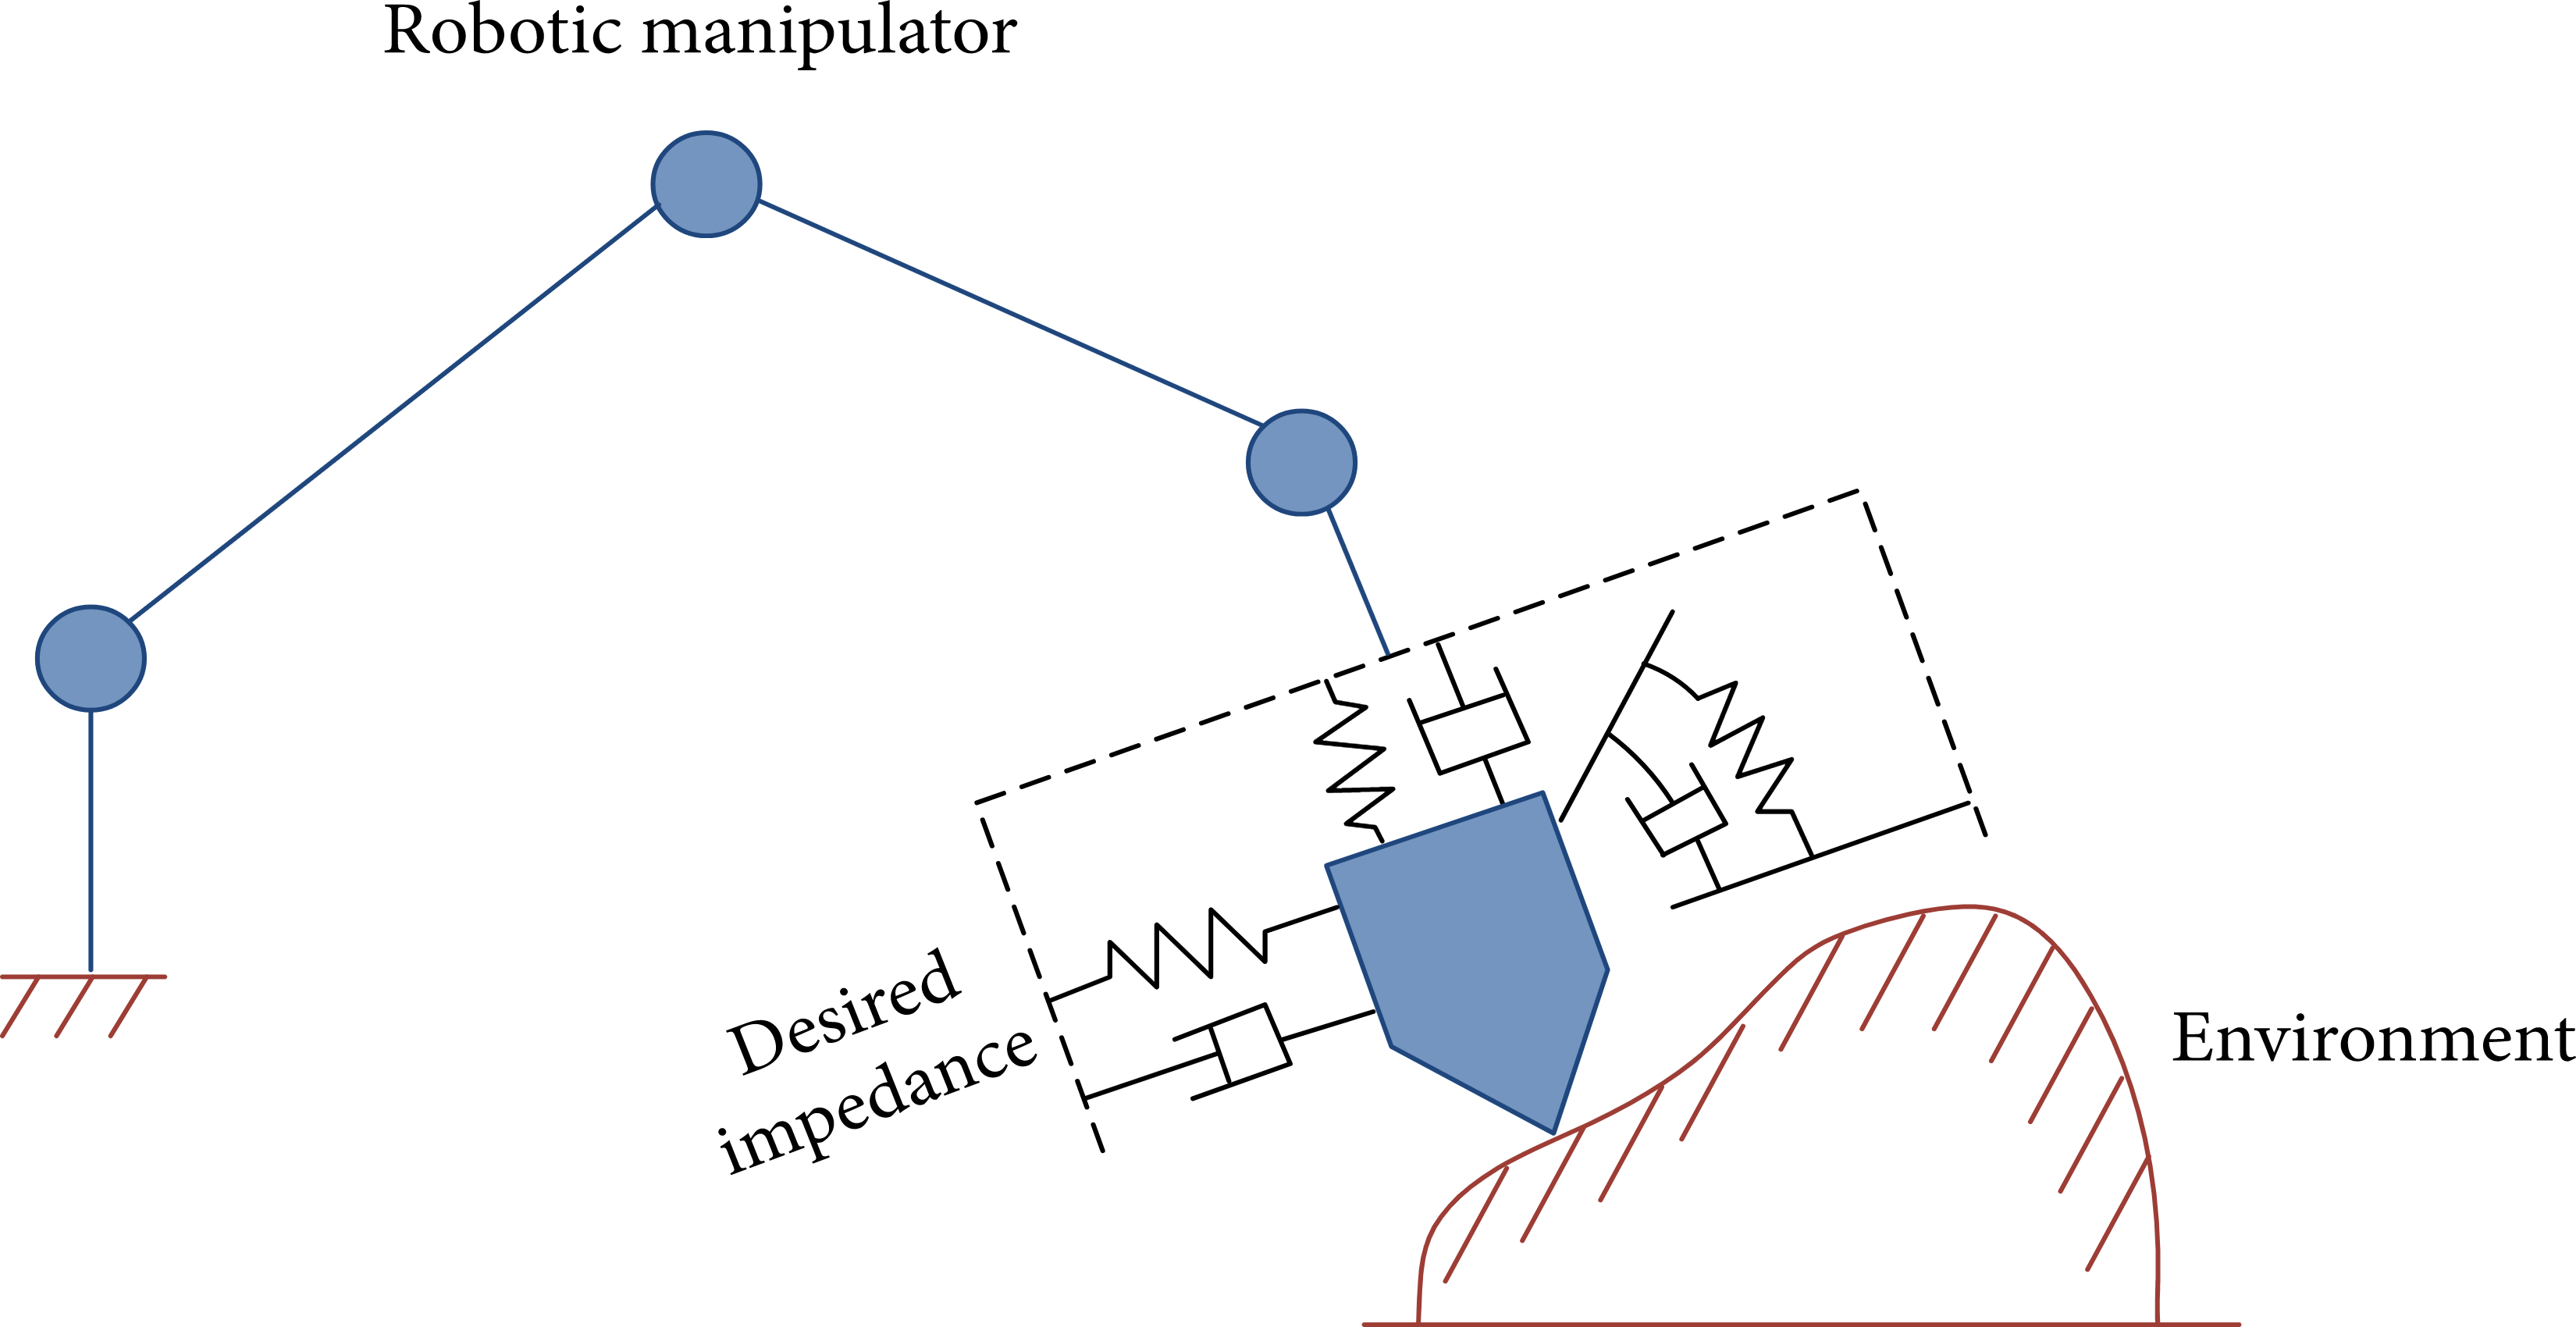
\includegraphics[width=0.5\linewidth]{figures/alshuka_2018.png}

  \caption[Impedance controlled manipulator in contact with the environment.]{Visual representation of impedance control in contact with the external environment \cite{al-shukaActiveImpedanceControl2018}.} \label{fig:impedance_control}
\end{figure}

In impedance control, the desired robot-environment interaction is modelled as a spring-damper system (see figure \ref{fig:impedance_control}) and is generally expressed\footnote{This relationship can also be expressed in the joint space \cite{tsetserukouISoRAHumanoidRobot2009,liImpedanceControlMultipoint2011,liModelfreeImpedanceControl2011,liLearningImpedanceControl2012}. This representation was omitted here since the cartesian version offers more intuition due to its close relationship to the task space.} as
\begin{equation} \label{eq:impedance_relationship}
  M_d \left(\ddot{ x }_e -\ddot{ x }_d \right)+ B_d \left(\dot{x}_e - \dot{x}_d \right)+ K_d \left( x_e - x_d \right) = M_d \ddot{\widetilde{ x }}+ B_d \dot{\widetilde{ x }}+ K_d \widetilde{ x }= F_a,
\end{equation}
in which $x_e$, $\dot{x}_e$, and $\ddot{ x }_e \in\mathbb{R}^n$ are the current position, velocity and acceleration of the manipulator's end effector in the cartesian coordinates, respectively, while the subscript $d$ denotes their desired values. Further, $F_a$ denotes the vector of external forces and torques affecting the system as expressed in the frame of the analytic Jacobian, and $M_d$, $B_{d}$ and $K_d \in\mathbb{R}^{ n \times n }$ are the inertia, damping and stiffness matrices of the desired impedance relationship, respectively, all of which are symmetric and nonnegative definite. This general impedance relationship, called the second-order impedance, can also be simplified to its first or zero-order form by setting the $\ddot{x}_d$ and $\dot{x}_d$ to zero, respectively.

This desired impedance relationship can be enforced on the environment interaction through feedback linearization. Feedback linearization, also called dynamic inversion control, is a control technique that transforms a nonlinear system into a linear system by cancelling out (or compensating) the nonlinear terms. The manipulator model in \eqref{eq:euler_lagrange_cartesian} can be feedback linearized in the cartesian space using the following control law:
\begin{equation} \label{eq:impedance_control_step1}
  u = J_ A^T \left( q \right)\left[ M_x \left( q \right) y + C_x \left( q ,\dot{ q }\right)\dot{ x }_e + g_x \left( q \right)- F_a \right].
\end{equation}
Applying this control law to \eqref{eq:euler_lagrange_cartesian} gives us a linear and decoupled closed-loop system
\begin{equation} \label{eq:impedance_control_step2}
  \ddot{ x }_e = y,
\end{equation}
where $y$ represents a new input vector that directly influences, with a double integrator, the independent cartesian coordinates $x$. This input allows us to enforce any dynamic relationship onto the controlled robot manipulator. By setting $y$ equal to
\begin{equation} \label{eq:impedance_control_step3}
  y = \ddot{ x }_d + M_ d^{- 1 }\left[- B_d \dot{\widetilde{ x }}- K_d \widetilde{ x }+ F_a \right],
\end{equation}
we end up with the impedance model given in \eqref{eq:impedance_relationship}. Combining and simplifying \eqref{eq:impedance_control_step3} and \eqref{eq:impedance_control_step1} gives us the general impedance control law:
\begin{equation}
  \begin{split}
    u = M \left( q \right) J_ A^{- 1 }\left( q \right)\left\{\ddot{ x }_d - \dot{ J }_A \left( q \right)\dot{ q } +  M_ d^{- 1 }\left[- B_d \dot{\widetilde{ x }} - K_d \widetilde{ x }\right]\right\} \\
    +\ C \left( q ,\dot{ q }\right)\dot{ q } + g \left( q \right) + J_ A^T \left( q \right)\left[ M_x \left( q \right) M_ d^{- 1 }- I \right] F_A.
  \end{split}
\end{equation}
This control law, sometimes called \textbf{torque-based impedance control}, produces forces in response to changes in motion and can, therefore, directly be applied to effort-controlled manipulators (see figure \ref{fig:force_based_impedance_control}) or through an optional inner force control loop \cite{al-shukaActiveImpedanceControl2018}. When an accurate model of the robot dynamics (i.e., $M \left( q \right)$, $C \left( q, \dot{ q }\right)$ and $g \left( q \right)$) and a measurement of the external forces and torques $F_a$ are available, it allows precise shaping of the environment interaction using the impedance parameters $M_d$, $B_d$, $K_d$. Of these, $M_d$ influences the control system's response speed, $B_D$ the shape of the transient behaviours and $K_d$ the trade-off between contact forces and free space position accuracy.

% FIGURE - Force-based impedance control schedule.
\begin{figure}
  \centering
  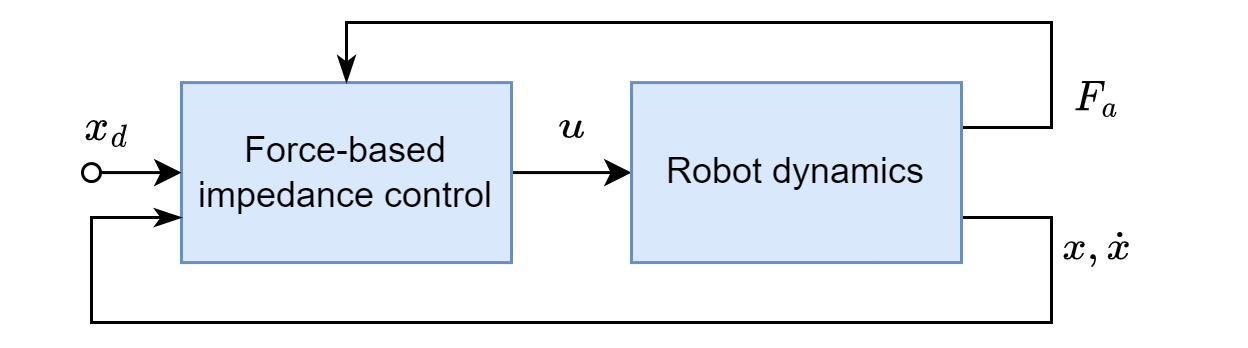
\includegraphics[width=0.65\linewidth]{figures/force_impedance.png}

  \caption[Force-based impedance control diagram.]{Schematic diagram of force-based impedance control. In this figure, $x$ and $\dot{ x }$ are the current position and velocity, respectively, $x_d$ is the desired position, $u$ the control command and $F_a$ the external forces and torques \cite{ottCartesianImpedanceControl2008}.} \label{fig:force_based_impedance_control}
\end{figure}

\subsubsection{Cartesian stiffness control}

The general impedance model above can only be used when a measurement of the external force $F_a$ is available. In some cases like robotic surgery, however, placing a force sensor at the robot end-effector can be difficult \cite{ferragutiTankbasedApproachImpedance2013}. It turns out that impedance control can also be used in these situations if we modify \eqref{eq:impedance_relationship} so that the desired inertia $M_d$ is equal to the actual inertia of the robot $M_x\left( q \right)$:
\begin{equation}
  M_x \left( q \right)\ddot{\widetilde{ x }}+ \left( B_d + C \left( q ,\dot{ q }\right)\right)\dot{\widetilde{ x }}+ K_d \widetilde{ x } = F_a,
\end{equation}
where $C \left( q ,\dot{ q }\right)$ was introduced to preserve the mechanical properties of the configuration-dependent inertia $M_x \left( q \right)$. Applying this new impedance model through feedback linearization results in the following control law:
\begin{equation}
  u = M\left(q \right)J_A^{-1}\left(q\right)\left\{\ddot{x}_d - \dot{J}_A \left(q\right)J_A^{-1}\left(q\right)\dot{x}_d\right\} + C \left(q,\dot{q}\right)J_A^{-1}\left(q\right)\dot{x}_d + g \left( q \right) - J_ A^T \left( q \right)\left[B_d\dot{\widetilde{ x }} + K_d \widetilde{ x }\right].
\end{equation}
This new control law, called \textbf{cartesian stiffness control}, is similar to a pure motion control law but designed to keep limited contact forces at the end-effector level. It no longer has a dependency on the contact forces $F_a$ and can therefore be used without a measurement of this force. However, it has two drawbacks: first, we lose the ability to change the system's behaviour using the desired inertia $M_d$, and second, because of the presence of the extra $C \left( q ,\dot{ q }\right)$, it can only be used at low velocities.

\subsubsection{Admittance control}

% FIGURE - Position-based impedance control schedule.
\begin{figure}
  \centering
  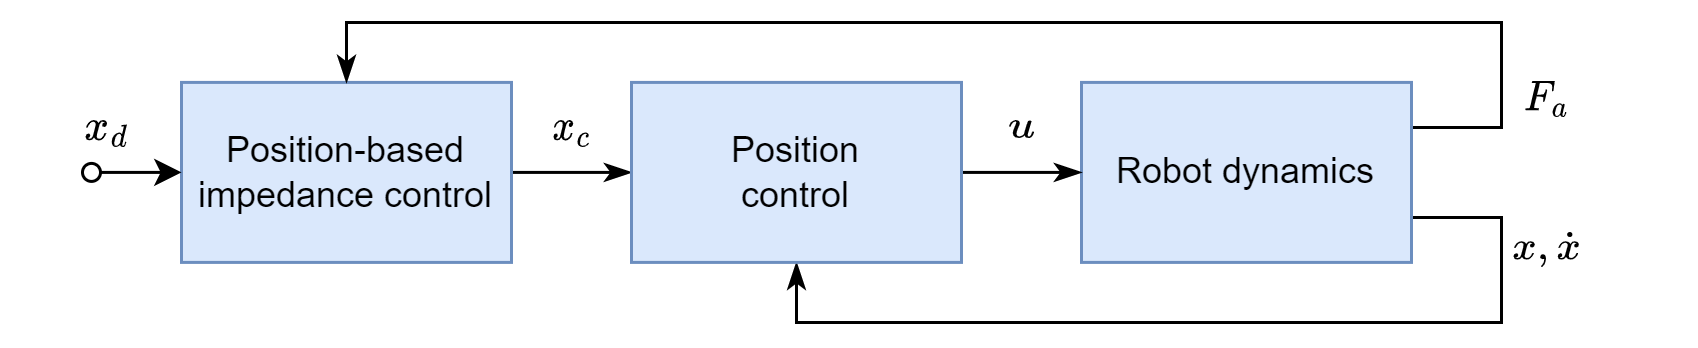
\includegraphics[width=0.9\linewidth]{figures/position_impedance.png}

  \caption[Position-based impedance control diagram.]{Schematic diagram of a position-based impedance controller. In this figure, $x$ and $\dot{ x }$ are the current position and velocity, respectively, $x_d$ is the desired position, $x_c$ the reference position, $u$ the control command and $F_a$ the external forces and torques \cite{ottCartesianImpedanceControl2008}.} \label{fig:position_based_impedance_control}
\end{figure}
As mentioned above, a trade-off exists between contact forces and free space position accuracy in general impedance control. In the absence of interaction (i.e., free motion), impedance control becomes equivalent to inverse dynamics position control, and therefore a high $K_d$ is needed for robustness against disturbances or model uncertainties. This high $K_d$ will, however, lead to undesired high impact forces when in contact. \textbf{Position-based or velocity-based impedance control} provides a solution to this trade-off by splitting the control into two control loops: an inner loop that controls (compliant) position or velocity references and an outer loop that provides these references based on the desired target impedance dynamics (see figure \ref{fig:position_based_impedance_control} for a general description). A simple proportional-integral-derivative (PID) can be used for the inner control loop, while a modified version of the impedance model in \eqref{eq:impedance_relationship} is used for the outer control loop:
\begin{equation}
  M_d \left(\ddot{ x }_c -\ddot{x}_d \right)+ B_d \left(\dot{ x }_c - \dot{ x }_d \right)+ K_d \left( x_c - x_d \right)= F_a,
\end{equation}
where $x_c$, $\dot{ x }_c$, and $\ddot{ x }_c \in\mathbb{R}^n$ now are the reference position, velocity and acceleration, respectively. This type of control, which generates reference motions $x_c$ in response to contact forces $F_a$, is also known as \textbf{admittance control} because of its close resemblance to mechanical admittance. It is often used for interaction tasks dealing with compliant environments or free space, while impedance control is often used for interactions with stiff environments.

\subsubsection{Variable impedance control (VIC)}
\label{section:variable_impedance_control}

Although the general impedance model in \eqref{eq:impedance_relationship} allows us to design the interaction with the environment precisely, it is still restrictive since this interaction can not be changed during the motion. It is therefore only suited for simple tasks where the environment stiffness is constant and can not be used to track desired contact forces. In contrast, humans change their muscle stiffness during motion to attenuate any disturbances or track desired interaction forces \cite{tomoriVariableImpedanceControl2013}. Doing this allows them to perform complex interaction tasks in changing and uncertain environments while precisely controlling the force applied to these environments. The general impedance model in \eqref{eq:impedance_relationship} can be extended to match this human behaviour by allowing the impedance parameters $M_d$, $B_d$ and $K_d$ to vary. This results in the following impedance model:
\begin{equation} \label{eq:variable_impedance}
  M_d\left(t \right)\ddot{\widetilde{ x }} + B_d \left( t \right)\dot{\widetilde{ x }} + K_d \left( t \right)\widetilde{ x }= F_a,
\end{equation}
in which the impedance parameters $M_d \left( t \right), \ B_d \left( t \right)\ and\ K_d \left( t \right)$ are now a function of time. As stated in the introduction, however, this \textbf{VIC} model destroys the passivity of the system unless a proper impedance profile is selected. To prove this, let us assume the desired inertia $M_d$ is constant while the desired damping $B_d$ and stiffness $K_d$ are allowed to change with time. Using the following positive definite Lyapunov function:
\begin{equation}
  V \left(\widetilde{ x }, \dot{\widetilde{ x }}\right)=\frac{ 1 }{ 2 }{\dot{\widetilde{ x }}}^T M_d \dot{ x }+\frac{ 1 }{ 2 }{\widetilde{ x }}^T K \left( t \right)\widetilde{ x }
\end{equation}
and taking its derivative while substituting $\ddot{ x }$ from \eqref{eq:variable_impedance} gives
\begin{equation} \label{eq:variable_impedance_derivative}
  \dot{V} = \dot{\widetilde{x}}^T F_a + \left[\frac{1}{2}\widetilde{x}^T \dot{K_d}\left(t \right)\widetilde{ x }-\dot{\widetilde{ x }}^T B_d \left( t \right)\dot{\widetilde{ x }}\right].
\end{equation}
From this derivative, since the sign of the term between the brackets is undefined, it is apparent that the passivity condition of definition \ref{def:passivity} only holds when the stiffness is constant or decreasing $\dot{V} \le \dot{\widetilde{x}} F_a$. As a result, energy might be injected into the system when the stiffness increases, possibly making it unstable. A similar conclusion can be drawn for the case where the inertia is also allowed to vary.

\subsection{Limitations}

While the indirect force control methods above, compared to direct force control methods, are better suited to handle interaction tasks, they also have one major drawback. Due to the use of feedback linearization, an accurate model of the system is required. They are therefore not suited in situations where this model is unavailable or significantly impacted by model uncertainties, disturbances or other noises. If this is the case, more advanced indirect control methods like robust or adaptive impedance control can be used \cite{songTutorialSurveyComparison2019,khalilNonlinearControl2015,villaniForceControl2016}.

\section{Further reading}

This chapter is intended to be a quick primer on stability, passivity, and impedance control. Readers can check out \cite{bacciottiStabilityControlLinear2019} for more information on stability criteria and control methods used with linear systems. For nonlinear systems, an excellent introduction to the control of nonlinear systems is given by \cite{khalilNonlinearControl2015}, while \cite{khalilNonlinearSystems2002} serves as a deep dive into all the stability proofs and more advanced methods. Further, \cite{baoProcessControlPassive2007} is an excellent introduction to passivity-based control, while \cite{haddadNonlinearDynamicalSystems2011} covers more advanced concepts. Lastly, readers are referred to \cite{sicilianoRoboticsModellingPlanning2010} for a detailed explanation of impedance control, while recent reviews of impedance research are found in \cite{songTutorialSurveyComparison2019} and \cite{al-shukaActiveImpedanceControl2018}.

\chapter{Stability methods in classical variable impedance control}
\label{chapter:classical_variable_impedance}

As shown in section \ref{section:variable_impedance_control}, the beneficial passivity property of constant (or fixed) impedance controllers no longer holds for variable impedance controllers, meaning the system can become unstable due to the control. Since no closed-loop solution exists for most interaction tasks, a classic stability analysis cannot be applied as the environment model is unknown or uncertain. Therefore, most authors have resorted to Lyapunov's stability theory and the concept of passivity to prove that systems controlled by variable impedance stay stable when interacting with these unknown environments. In the literature, two main groups of methods can be found for ensuring the stability of variable impedance controllers: Solutions that try to enforce the passivity online through \textbf{pacifying control algorithm} and solutions that use \textbf{stability constraints} to ensure the passivity of a given controller or impedance profile offline. The following sections discuss the methods used with classical variable impedance controllers like adaptive and optimal controllers. The methods used in learning-based variable impedance controllers are described in the next chapter. Although this review focuses on stability, some mechanisms for ensuring safety are also briefly mentioned below to aid the understanding of the shortcomings of specific passivity methods.

\section{Pacifying control algorithms}

\subsection{Energy-tanks}

One of the first authors to use a pacifying control algorithm for creating a stable variable impedance controller was Ferraguti et al. \cite{ferragutiTankbasedApproachImpedance2013}. By looking at the passivity condition derived for the constant impedance controller (i.e., equation \eqref{eq:variable_impedance_derivative}\footnote{The passivity condition for a constant impedance controller is obtained from equation \eqref{eq:variable_impedance_derivative} by setting $\dot{K}_d$ equal to zero.}), they realised that the dissipation term serves as a passivity margin. The more power dissipated in the system, the stricter the passivity condition becomes, and the more the desired stiffness can be adjusted without threatening the passivity of the closed-loop system. Therefore, by augmenting the impedance model with an energy-storing element, a tank, they could track the dissipated energy to be later used to implement the VIC. While doing this, a tank upper limit is set to avoid potentially hazardous situations, and a constant stiffness is used to maintain the closed-loop system's passivity when the energy in the tank is almost empty. This strategy was later extended in \cite{ferragutiEnergyTankBasedInteractive2015} to work with second-order impedance control algorithms that vary not only the desired stiffness but also the desired damping and inertia.

Several works have used this strategy to ensure passivity while varying impedance through adaptive or optimal control \cite{cordoniVariableStochasticAdmittance2020,dietrichPassivationProjectionBasedNull2016,dietrichPassiveHierarchicalImpedance2017,michelPassivitybasedVariableImpedance2020,chenDrawingElonMusk2021,balattiMethodAutonomousRobotic2020,scibiliaSelfAdaptiveRobotControl2018,selvaggioPassiveVirtualFixtures2018,tadeleCombiningEnergyPower2014,karacanPassivityBasedSkillMotion2022}. Although theoretically sound from an energy perspective, this method has three main shortcomings:
\begin{enumerate}
    \item A singularity exists when the energy tank is empty. As a result, the tank has to be initialised with a certain amount of energy before the control action. This initialisation will make the controller more complex and worsen the performance.
    \item The control performance depends on the tank's initial energy and upper energy bound. These values must be correctly tuned to guarantee a particular variable impedance profile. If the initial energy accumulated in the tank is too low, the controller will run out of energy before the variable impedance profile is completed. If the upper bound is too high, the controller might release too much energy at once, leading to fast and unsafe behaviours.
    \item It depends on the current robot state and can only be applied online. Consequently, the execution of a desired variable impedance profile cannot be guaranteed beforehand because a constant stiffness is used when the tank is almost empty.
\end{enumerate}

To solve the first shortcoming, Zheng et al. \cite{zhengTimeVaryingImpedanceControl2018} modified the energy tank formula with an exponential so that the singularity does not occur anymore when the tank is empty. Saudrais et al. \cite{saudraisRateModeBilateral2021}, on the other hand, use a progressive damping injection mechanism to ensure the tank never becomes empty. This mechanism slightly increases the damping parameter to add energy to the tank when the lower limit is reached and decreases it again when the upper bound is reached. Lastly, Secchi et al. \cite{secchiEnergyOptimizationRobust2019} reframed the original impedance control problem as a constraint convex optimisation problem, in which the minimum tank energy is constrained to be above a specific limit. They solve this problem online to retrieve the variable impedance behaviour that best approximates the desired impedance behaviour without depleting the tank. Since their method plans the (passive) control behaviour closest to the desired one, they prevent the singularity from occurring while also improving the performance. This method was later generalised by Capelli et al. \cite{capelliPassivityControlBarrier2022}, who encoded the passivity and minimum tank energy constraints of \cite{secchiEnergyOptimizationRobust2019} as a Control Barrier Function (CBF) \footnote{Similar to a CLF, but instead of guaranteeing that a trajectory converges to a particular stable set, it ensures it can never leave a particular safe set (i.e., a desired constraint is always satisfied)  \cite{amesControlBarrierFunctions2019}.}. Using this CBF, their method applies to a broader range of control systems. Additionally, it leads to a more gradual enforcement of the passivity and minimum energy constraints, resulting in better tracking performance.

% NOTE: Schindlbeck et al. 2015, Shahriari et al. 2018/2020 use constant impedance but is added here since it can also be applied to variable impedance.
% NOTE: Shahriari et al. 2018 uses DMP. Mentioned here since this DMP is programmed and not learned and the technique is applicable to variable impedance.
% NOTE: Here I also included safety mechanisms since I already this section before I decided to only focus on stability.
For the second shortcoming, several solutions have been proposed. Schindlbeck et al. \cite{schindlbeckUnifiedPassivitybasedCartesian2015}, for example, estimate the energy needed to fulfil the desired task using a linear reaction force model and apply it to the tank to ensure enough energy is in the tank to complete this task. While doing so, a configuration-dependent shaping function on the controller output is used to prevent fast and unsafe behaviour at contact loss. Gerlagh et al. \cite{gerlaghEnergyawareAdaptiveImpedance2021} take a slightly different approach by recovering the required task energy using an offline optimisation. They do not set this energy at the start but gradually release it throughout the motion to ensure the control behaviour is safe. Finally, to prevent the fast and unsafe behaviours mentioned above, Shahriari et al. 2018, 2020 \cite{shahriariValvebasedVirtualEnergy2018,shahriariPowerFlowRegulation2020,michelSafetyAwareHierarchicalPassivityBased2022} limit the power exchanged from the tank at any given time. Shahriari et al. \cite{shahriariValvebasedVirtualEnergy2018} accomplish this by adding adjustable valves into the tank design, which can control the power released during the task execution. Later, in Shahriari et al. \cite{shahriariPowerFlowRegulation2020}, these valves are replaced by a constraint that directly enforces a specific power exchange profile on the output of the energy tank. This power flow regulation mechanism was used in a later paper by Michel et al. \cite{michelSafetyAwareHierarchicalPassivityBased2022} to satisfy a maximum kinetic energy constraint, thereby ensuring that collisions do not lead to injuries.

\subsection{Potential fields}

While the methods above solve the first two shortcomings of the original energy tank, they significantly complicate the controller design, rely on additional interaction models, slow down the control frequency or hurt the system performance. More importantly, their effectiveness depends on the ability to track the energy dissipated in the system, and their performance cannot be guaranteed for highly-variable environments that might consume all tank energy. As a result, Babarahmati et al. \cite{babarahmatiFractalImpedancePassive2021} replaced the energy tank with an asymptotic stable potential field called a fractal attractor (FA). This FA is used to encode the convergence and divergence behaviour of the variable impedance controller. It accumulates the potential energy of the controller when diverging from the desired state so that it can later be used to converge back to this state passively. In their paper, Barbarahmati combines this FA with a cartesian stiffness controller to form a new (passive) variable impedance controller called a Fractal Impedance Controller (FIC). They use this FIC to execute a nonlinear state-dependent variable stiffness profile. This profile can be changed online to enforce a desired impedance relationship without affecting the system's stability, thus guaranteeing stable interaction with unknown environments. Unlike the original energy tank, this new FIC does not need energy dissipation tracking or an energy initialisation method. It also does not rely on energy damping to dissipate energy, achieves a better control performance, and is intrinsically robust against discretisation, model errors, and noise because it is path-independent. It, however, contains a non-smooth force transition while switching from divergence to convergence, which can hurt control performance. Tiseo et al. \cite{tiseoBiomimeticAdaptiveForce2020} solved this problem by replacing the simple stiffness profile used in \cite{babarahmatiFractalImpedancePassive2021} with a more flexible force profile. This new profile simplifies the controller's tuning for different tasks, and more importantly, it results in a smooth force transition between convergence and divergence. In addition, a force-feedback loop was also added to the FIC, enabling it to be used with force sensing or tracking tasks such as haptic exploration. Since then, this (improved) FIC has been deployed successfully in several manipulation and teleoperation tasks \cite{tiseoRobustImpedanceControl2022,tiseoFineManipulationDynamic2022,tiseoAchievingDexterousBidirectional2022,tiseoGeometricalPosturalOptimisation2022,babarahmatiRobustHighTransparencyHaptic2021,tiseoSafeCompliantControl2020}.

\subsection{Stability constraints}

Although potential fields solve most of the shortcomings of the original energy tank, they are still state-dependent. As a result, they, like energy tanks, are unsuitable for guaranteeing the execution of a desired variable impedance profile in advance. Several authors have therefore used a Lyapunov stability analysis to derive constraints that ensure the stability of their adaptive controllers \cite{leeForceTrackingImpedance2008,linUnifiedMotionForce2021,maFractionalorderSlidingMode2019,maVariableStiffnessDamping2019,sunModelReferenceAdaptive2021,yangHumanlikeAdaptationForce2011,wahballaConstantForceTracking2022,liForceImpedanceTrajectory2018,hamedaniIntelligentImpedanceControl2021,hamedaniRecurrentFuzzyWavelet2021,ganeshVersatileBiomimeticController2012}. These stability constraints are, however, controller specific and can not be used to prove the stability of a general variable impedance profile. Therefore, a paper by Kronander et al. \cite{kronanderStabilityConsiderationsVariable2016} performed a Lyapunov stability analysis on the general variable impedance controller. Using a Lyapunov candidate function, they derived a \textbf{state-independent} stability constraint that relates the desired stiffness and its time derivative to the desired damping. This constraint can be used \textbf{offline} to verify a system's (asymptotic) stability for a given impedance profile or directly incorporated into an optimization or learning procedure. The resulting profiles can then be executed with any standard impedance control architecture while ensuring the (perturbed) system cannot go unstable, guaranteeing accurate trajectory tracking in free motion. Alternatively, it can also be implemented as a passivity filter that modifies non-passive impedance profiles \textbf{online} such that the passivity of the closed-loop system is guaranteed \cite{bednarczykPassivityFilterVariable2020}.

Several papers have used the constraint of Kronander et al. \cite{kronanderStabilityConsiderationsVariable2016} with adaptive or optimal control-based variable impedance controllers to ensure the stability of the control \cite{fontanelliComparisonAssistiveMethods2018,liuAdaptiveEnhancedAdmittance2022,liangAdaptiveTimeVaryingImpedance2022,heVariableImpedanceControl2020,dongAdaptiveStiffnessDamping2019}. Even though the constraint above guarantees the stability of the control in a state-independent way it has several limitations. First, because the constraint is very conservative, some stable impedance profiles may be incorrectly classified as unstable, causing the tracking performance to be significantly impacted. To improve this, Bednarczyk et al. \cite{bednarczykPassivityFilterVariable2020} proposed another Lyapunov candidate function that leads to a less conservative stability constraint. Second, the original constraint does not consider external forces in the stability analysis. As a result, the stability of the control system is only guaranteed under the assumption of a free, unconstrained motion. Several papers have, however, derived similar stability constraints on the desired variable impedance dynamics for which stability of the unconstrained motion (i.e. AS and ES) and passivity or ISS of the constraint motion is proven
\cite{parkInputtoStateStabilityVariable2020,sunStabilityGuaranteedVariableImpedance2021,zhangNeuralApproximationbasedAdaptive2020,bednarczykPassivityFilterVariable2020}. Lastly, the constraint derived by Kronander et al. \cite{kronanderStabilityConsiderationsVariable2016} assumes that the desired inertia remains constant, which requires correct model knowledge, dynamic decoupling, and external force measurement. As a result, the constraint cannot be used with methods that vary the desired inertia or methods that set the desired inertia equal to the configuration-dependent robot inertia, such as Cartesian stiffness control. To solve this, Dong et al. \cite{dongUDEBasedVariableImpedance2019} derived a stability constraint on the desired stiffness, damping, and inertia that can be used to ensure the control system's passivity when all impedance parameters are varied. Further, a paper by Park et al. \cite{parkInputtoStateStabilityVariable2020} derived a stability constraint that incorporates the configuration-dependent robot inertia and can therefore be used to guarantee ISS of a Cartesian stiffness controller.

\chapter{Stability methods in learning based variable impedance control}
\label{chapter:learning_based_variable_impedance}

% TODO: Seperation not correct see Abu-dakka

The previous chapter discussed methods for ensuring stable control in classical variable impedance controllers. Although impressive results were achieved using these classical controllers \cite{songTutorialSurveyComparison2019}, these controllers' variable impedance profiles are manually programmed for a given task. This considerably reduces the usability of these controllers since every time a robot is used for a new task, multiple hours of labour by skilled workers are required for re-programming the controller. In recent years, numerous authors have instead switched to learning-based variable impedance controllers \cite{abu-dakkaVariableImpedanceControl2020}. These controllers allow learning more complex behaviours without requiring the researcher to program this behaviour explicitly. A recent review of these learning-based variable impedance controllers was done by \cite{abu-dakkaVariableImpedanceControl2020}. In this review, the learning-based VIC methods were classified into two main groups: Variable Impedance Learning (VIL), in which the impedance profiles are learned from human demonstrations (through imitation learning) to be later executed with an existing impedance controller, and Variable Impedance Learning Control (VILC) in which the impedance control law is directly learned (through imitation learning, iterative learning or reinforcement learning). Where \cite{abu-dakkaVariableImpedanceControl2020} focuses on the learning-based VIC methods used in the current literature, the following sections concentrate on the stability and passivity techniques employed to ensure stability while using these methods.

\section{Variable impedance learning}

\subsection{Stability of the learned trajectories}

As explained above, in VIL methods, the desired trajectory and impedance profiles for a given task are learned from human demonstrations using a supervised learning procedure called Imitation Learning (IM), also called Learning from Demonstrations (LfD). Two steps generally make up this approach: A step in which kinematic (and dynamic) data is collected from sensors (i.e. data-collection step), followed by a step in which a model is fitted to the collected data using regression (i.e. data-fitting step). Depending on the task, any regression model (e.g. linear models, splines, gaussian mixture models, neural networks, gaussian processes) and accompanying regression technique can be used in this data-fitting step \cite{kroemerReviewRobotLearning2021,husseinImitationLearningSurvey2017}. Traditionally, LfD research has mainly focused on reproducing the demonstrations' kinematics (i.e. trajectories) \cite{siReviewManipulationSkill2021}. At first glance, this trajectory reproduction problem seems to be a simple regression task that can be solved by minimising the squared distance between the sampled trajectories and the regression model. A low-level controller like a PID controller can then be used to reproduce the recorded trajectories. However, in practice, such a naive regression approach has proven to be insufficient because it results in an over-fitted model that does not generalise outside of the demonstrated trajectories \cite{sindhwaniLearningContractingVector2018}. Therefore, this (nonlinear) model is only locally stable and does not converge to the desired trajectories if situations are encountered that were not present in the training data (e.g. different initial states, temporal disturbances and spatial disturbances). One possible solution would be to use linear regression models in which stability outside the demonstrated regions can be proven easily. Such models, however, cannot accurately reproduce desired trajectories that are nonlinear and non-smooth. Therefore, several methods have been proposed in the literature for learning (nonlinear) trajectories while guaranteeing stability outside the demonstrated region.

In LfD research, motions are often modelled as a Dynamic System (DS) \cite{khansari-zadehLearningStableNonlinear2011} to improve generalizability. Compared to classical approaches, which use time-indexed trajectories, in a DS, the trajectories are formulated as a differential equation. Because of this, the DS captures both the trajectories and the essential dynamics that underlie a given task, making it better able to adapt to environmental changes like temporal and spatial disturbances. The most widely used DS-based approach for learning stable nonlinear trajectories is the so-called "Dynamic Movement Primitives" (DMPs) \cite{ijspeertDynamicalMovementPrimitives2013,saverianoDynamicMovementPrimitives2021,wangLearningDemonstrationUsing2021,sidiropoulosReversibleDynamicMovement2021,ginesiOvercomingDrawbacksDynamic2021,rozanecNeuralDynamicMovement2022,liProDMPsUnifiedPerspective2022}. In DMPs, a globally stable linear DS is coupled with a nonlinear forcing term through a phase variable to create an autonomous, weakly nonlinear DS. This DS can learn complex high-dimensional motions from single \cite{ijspeertDynamicalMovementPrimitives2013,prakashDynamicTrajectoryGeneration2020} or multiple demonstrations \cite{matsubaraLearningParametricDynamic2011,pervezLearningTaskparameterizedDynamic2018} while guaranteeing global stability. This global stability is achieved by exponentially or linearly decaying the phase variable during the task, thereby decreasing the effect of the possibly unstable nonlinear forcing term. As these DMPs are time- and scale-invariant, the learnt motions' velocity and amplitude can be scaled without losing stability, making them well-suited for reacting to external perturbations in real-time. Unfortunately, although the phase variable ensures the stability of the motions, it introduces an implicit time dependency in the DMP formulation. Due to this time dependency, the motion of the DMP is very dependent on the phase variable, which is, again, task-dependent. Consequently, DMPs have poor generalisation capabilities outside the demonstrations and are not robust against temporal disturbances \cite{neumannLearningRobotMotions2015}.

Other authors use a constraint optimisation approach to overcome the abovementioned limitations and encode the demonstrated motions in a state-dependent nonlinear DS while enforcing global stability through Lyapunov constraints. Since these DSs are time-independent, the learned policies are now robust against temporal disturbances. This was first done by Khansari-Zadeh et al. \cite{khansari-zadehLearningStableNonlinear2011}, who introduced a stable estimator of a dynamical system (SEDS). By limiting the parameters of a Gaussian mixture regression model (GMM) using a Quadratic Lyapunov constraint, SEDS can learn accurate motions while guaranteeing global stability. Similar Lyapunov constraints were used in literature with other regression models to ensure the global stability of the learned motions \cite{lemmeNeurallyImprintedStable2013,huNeuralLearningStable2015,umlauftLearningStableStochastic2017,umlauftLearningStableGaussian2017,medinaLearningStableTask2017,duanFastStableLearning2019,xuRobotTrajectoryTracking2019,umlauftLearningStochasticallyStable2020,ledererGaussianProcessBasedRealTime2021,xuLearningBasedKinematicControl2022,salehiLearningDiscreteTimeUncertain2022,davoodiRuleBasedSafeProbabilistic2022}. Unfortunately, as these methods' stability criteria are derived based on a simple quadratic Lyapunov function, they can only model trajectories in which the distance to the target decreases monotonically in time, leading to poor accuracy if demonstrated trajectories are not contractive. As a result, several authors have used parametric and non-parametric Lyapunov candidates to learn less conservative Lyapunov constraints directly from data to improve this so-called accuracy-stability dilemma \cite{mohammadkhansari-zadehLearningControlLyapunov2014,neumannNeuralLearningStable2013,lemmeNeuralLearningVector2014,umlauftLearningStableGaussian2017,umlauftUncertaintybasedControlLyapunov2018,duttaLearningStableMovement2018,umlauftUncertaintybasedHumanMotion2019,duttaSkillLearningHuman2021,ravanbakhshLearningControlLyapunov2019,ravanbakhshFormalPolicyLearning2019,umlauftLearningStochasticallyStable2020,xiaoLearningStableNonparametric2020,tesfazgiInverseReinforcementLearning2021,coulombeGeneratingStableCollisionFree2022,jinLearningNeuralshapedQuadratic2023}. These less conservative Lyapunov constraints can then be enforced \textbf{offline} during learning or \textbf{online} through a stabilising control command to ensure the stability of the reproduced trajectories. If applied online \cite{mohammadkhansari-zadehLearningControlLyapunov2014,umlauftLearningStableGaussian2017,umlauftUncertaintybasedControlLyapunov2018,duttaLearningStableMovement2018,umlauftUncertaintybasedHumanMotion2019,ravanbakhshFormalPolicyLearning2019,ravanbakhshLearningControlLyapunov2019,xiaoLearningStableNonparametric2020,duttaSkillLearningHuman2021,umlauftLearningStochasticallyStable2020}, any regression method can be used. However, no guarantees can be given about the accuracy of reproduced trajectories since the control command potentially interferes with the dynamic system. If applied offline \cite{neumannNeuralLearningStable2013,lemmeNeuralLearningVector2014,tesfazgiInverseReinforcementLearning2021,coulombeGeneratingStableCollisionFree2022,jinLearningNeuralshapedQuadratic2023}, on the other hand, the shape and accuracy of the demonstrated trajectories are known beforehand, but the implementation is specific to the used regression model. This significantly restricts the applicability of these offline methods since it is unknown beforehand which regression technique would be more effective for a given task.

Although the learned Lyapunov constraints above yield more accurate motions than their fixed counterparts and DMPs, finding them is more computationally intensive and time-consuming. Furthermore, their reproduction accuracy still depends on the Lyapunov candidate function used during learning. While less conservative Lyapunov candidate functions could be used to improve the accuracy of the reproduced trajectories, finding these Lyapunov candidate functions is not easy, time-consuming, and quickly becomes computationally intractable \cite{ravanbakhshLearningControlLyapunov2019,havensImitationLearningLinear2021,tesfazgiInverseReinforcementLearning2021}. Additionally, except \cite{jinLearningNeuralshapedQuadratic2023}, all of the offline methods of the previous paragraph currently lack constructive mathematical guarantees causing the stability of these methods to be restricted to finite regions in the workspace. Therefore, these methods only apply to applications where the task region is bounded and known a priori. Because of this, recent papers have taken a diffeomorphic approach and transformed the demonstrations into a latent space in which the demonstrations are consistent with a (simpler) predefined or learned Lyapunov function \cite{neumannLearningRobotMotions2015,perrinFastDiffeomorphicMatching2016,jinLearningAccurateStable2019,ranaEuclideanizingFlowsDiffeomorphic2020,gaoLearningDynamicalSystem2021,urainImitationFlowLearningDeep2020,takeishiLearningDynamicsModels2021,ficheraLinearizationIdentificationMultipleAttractor2022,guptaLearningHighDimensional2022,zhiDiffeomorphicTransformsGeneralised2022,zhangLearningAccurateStable2022,saverianoLearningStableRobotic2022,urainLearningStableVector2022,wangLearningDeepRobotic2022,zhangLearningRiemannianStable2022}. By enforcing the Lyapunov constraints in this new latent space, the global stability of the learned motions can be guaranteed offline. Since this latent space, which can be of the same or a higher dimension, is topological equivalent to the original space, the stability achieved in this space is retained when the learned demonstrations are eventually transformed back to the original space \cite{leeIntroductionTopologicalManifolds2011,leeIntroductionSmoothManifolds2012,leeIntroductionRiemannianManifolds2018}. Although a transformation that preserves stability has to be found, finding this transformation is relatively easier than finding a suitable Lyapunov function in the untransformed space. As a result, compared to previous methods, these diffeomorphic methods can handle more complex high-dimensional motions with less computational effort. Research has learned that diffeomorphic methods exhibit better reproduction accuracy and generalizability since they can learn a more general group of demonstrations than the abovementioned methods. However, they introduce more tunable parameters, can currently only be used offline and are specific to the used regression technique. Moreover, the expressiveness of the function approximator used for the diffeomorphic transform determines the accuracy and generalizability of these methods.

The methods discussed above were able to achieve high accuracy while guaranteeing the stability of the equilibrium points. They, however, give no guarantee about the convergence of the trajectories. As a result, although learned policies will always reach the target, regardless of the region in the state space where they are perturbed, they will no longer follow the reference trajectories. These techniques are, therefore, inadequate for tasks where trajectory tracking is crucial. Because of this, several authors have used contraction theory to derive stability constraints that guarantee a "stronger" type of stability called incremental stability. Instead of looking at the stability of the equilibrium points, incremental stability studies the convergence between any two trajectories of a given system \cite{lohmillerContractionAnalysisNonlinear1998,tsukamotoContractionTheoryNonlinear2021}. These (incremental) stability constraints have been used \textbf{offline} \cite{ravichandarLearningContractingNonlinear2016,ravichandarLearningStableNonlinear2018,khadirTeleoperatorImitationContinuoustime2019,sindhwaniLearningContractingVector2018,ravichandarLearningPositionOrientation2019} and \textbf{online} \cite{blocherLearningStableDynamical2017} with different regression models to improve the accuracy of the reproduced trajectories. Contraction-based methods have shown better or similar results to the diffeomorphic methods above. However, since their contraction-based constraints lead to exponential stable DSs, they provide greater robustness against temporal and spatial perturbations \cite{ravichandarLearningPartiallyContracting2017}. Nonetheless, the robustness and accuracy of these methods are highly dependent on the contraction metrics used to derive these constraints. Furthermore, only a small class of contraction metrics (i.e. positive definite symmetric matrices and a sum of squares polynomials) are currently used in literature and deriving them is non-trivial and dependent on the used regression model. Additionally, due to their inherent contractive nature, these approaches, however, suffer from the risk of over-corrections, making them unsuited for tasks containing global or locally divergent trajectories \cite{figueroafernandezPhysicallyconsistentBayesianNonparametric2018,figueroaLocallyActiveGlobally2022}. Several papers have recently combined contraction theory and diffeomorphisms with global linearization methods inspired by Koopman theory to solve these issues \cite{bevandaKoopmanOperatorDynamical2021}. These Koopman-based approaches work by mapping the system states of the nonlinear system to high (possibly infinite) dimensional spaces of observables
in which the dynamics are linear. A globally linear representation of the original nonlinear system can be achieved by learning these Koopman observables and the accompanying mapping from data. Contraction theory can then be used on this representation to guarantee the global stability of the original nonlinear system. These Koopman-based methods, like the diffeomorphic methods above, lead to more challenging system identification but make it easier to guarantee global stability. Even though these methods have shown good accuracy and robustness in simple learning from demonstration datasets \cite{fanLearningStableKoopman2021,bevandaDiffeomorphicallyLearningStable2022}, they are relatively new and yet to be compared to the methods above on more complex LFD tasks.

Lastly, two other noteworthy approaches for guaranteeing stability in kinematic LfD research are found in the current literature. The first one, a paper by Savariano et al. \cite{saverianoEnergybasedApproachEnsure2020}, used the energy tank of the previous chapter to ensure the DS's stability \textbf{online}. By storing the energy of stable (conservative) actions in this tank, potentially unstable motions can be performed as long as there is enough energy in the tank, thereby preserving the system's overall stability. Their method can achieve comparable accuracy as the aforementioned constrained-based methods, can be used with any regression technique, is less computationally intensive and requires fewer parameters to be tuned. However, it has an implicit time dependency and, like the energy tank-based methods in the previous chapter, requires a tank initialisation procedure which can significantly affect the reproduction accuracy. The second one, a paper of Figueroa et al. \cite{figueroafernandezPhysicallyconsistentBayesianNonparametric2018}, used a non-parametric GMM to learn the movement policy and an elliptical Lyapunov function jointly. They introduce a novel similarity metric which leverages locality and directionally of the demonstrations and use this metric as a Bayesian prior in the constraint optimisation. By doing this, they end up with a globally asymptotically stable DS that also converges locally to the demonstrated trajectories. Their algorithm outperforms several methods described earlier in accuracy and generalizability without relying on diffeomorphisms or contraction theory.

\subsection{Stability of the learned impedance}

% QUESTION: Are the papers of Jin et al. 2022, Duo et al. 2022, Duan et al. 2019 and Arduengo et al. 2020 also passive and thus IO stable? I think since Kronander et al. 2016 is used and they give no IO or passivity proof they are not. It could however be that my understanding of the problem is wrong.

The previous section depicted several solutions for learning stable kinematic motion from demonstrations. Since robotic manipulators seldom only perform movements in free space, researchers have augmented these methods for interaction tasks. Several papers, for example, have extended the original DMP model of the previous section with an additional forcing or coupling term that encodes the desired impedance behaviour \cite{saverianoDynamicMovementPrimitives2021,dongDMPbasedOnlineAdaptive2021,hanModifiedDynamicMovement2022,hanModifiedDynamicMovement2022,liaoDynamicSkillLearning2022,yangDMPsbasedFrameworkRobot2018,yuHumanRobotVariableImpedance2022,zengRobotLearningHuman2018,zhangLearningGeneralizingVariable2022}. Since both the kinematic and impedance terms are linked to the same exponentially decaying phase variable, the stability of the reproduced motions and impedance profiles is guaranteed. Other authors use the Lyapunov constraint-based approach from the previous section to ensure the stability of their learned variable impedance controllers. Some directly encode the impedance behaviour on a Riemannian manifold and use a diffeomorphic approach \cite{saverianoLearningStableRobotic2022,wangLearningDeepRobotic2022} while others use
stability constraints similar to those of Kronander et al. \cite{kronanderStabilityConsiderationsVariable2016} \cite{tangTeachIndustrialRobots2016,jinOptimalVariableImpedance2022,douRobotSkillLearning2022,duanSequentialLearningUnification2019,arduengoGaussianProcessbasedRobotLearning2020}. 

Although the stability of these impedance-based LfD methods in free motion is guaranteed, it does not imply passivity, and thus, the controlled system can become unstable when in contact. Therefore, several recent papers have focused on guaranteeing the passivity of these methods. In Khansari-Zadeh et al. \cite{khansari-zadehModelingRobotDiscrete2014}, both the motion and impedance control were encoded into a time-invariant DS, which was expressed as a nonlinear combination of a set of linear spring-damper systems. Stability constraints were derived by performing a passivity analysis on this DS to ensure free space stability and passivity in-contact \cite{khansari-zadehModelingRobotDiscrete2014}. This idea was further developed in \cite{khansari-zadehLearningPotentialFunctions2017}, where a non-parametric potential function and dissipative field were learned from demonstrations to encode the desired motion, stiffness and damping behaviour. The passivity and, thus, stability of this potential field-based variable impedance controller were demonstrated using a passivity analysis. Compared to \cite{khansari-zadehModelingRobotDiscrete2014}, this new method can model a more extensive range of motions, simplifies motion and impedance learning and allows explicit stiffness and damping adjustments without modifying the desired trajectory. Since then, multiple authors have used this method to ensure passivity \cite{wilzConstrainedHapticguidedShared2021,rossaRoboticRehabilitationAssistance2021,najafiUsingPotentialField2020,baiReachableWorkspaceRobotassisted2022,huFuzzyAdaptivePassive2023}. Instead, others have modified the energy-tank method given in the previous chapter to be used with LfD-based impedance controllers \cite{kronanderPassiveInteractionControl2016,shahriariAdaptingContactsEnergy2017}. Kronander et al. \cite{kronanderPassiveInteractionControl2016} designed a passive DS-based controller that can be used to learn motion and impedance control while ensuring stable interaction with a passive environment. The passivity and, thus, global stability of this controller is ensured through an energy-tank-like mechanism. This method was later extended by \cite{figueroaLocallyActiveGlobally2022,chenClosedLoopVariableStiffness2021} to encode locally contractive stiffness-like behaviours. Shahriari et al. \cite{shahriariAdaptingContactsEnergy2017}, on the other hand, augment the DMP approach from the previous section with a passivity observer, which modifies the phase variable when non-passive behaviour is detected. Ferraguti's energy tank is also added since this passivity observer merely reduces non-passive actions but does not guarantee passivity. Multiple authors have used these modified energy tank-based methods to ensure their learned controllers stay passive and thus stable during interaction tasks \cite{kastritsiPHRIFrameworkModifying2018,kastritsiProgressiveAutomationDMP2018,dimeasProgressiveAutomationPeriodic2020,papageorgiouKinestheticGuidanceUtilizing2020,krambergerPassivityBasedIterative2018,amanhoudDynamicalSystemApproach2019,enayatiVariableImpedanceForceControl2020,michelBilateralTeleoperationAdaptive2021,wuFrameworkAutonomousImpedance2021,wuLearningDemonstrationInteractive2022,zhaoHybridLearningOptimization2022}. Lastly, a paper by Franzese et al. \cite{franzeseILoSAInteractiveLearning2021} used a non-parametric model to learn stiffness and motion behaviour from human demonstrations. They use the uncertainty measure from the non-parametric model to create a potential field-like stability prior that steers motion back to regions where the model predictions have high confidence. Additionally, they decrease the stiffness to zero when the uncertainty becomes too large to prevent unstable behaviours. Although intuitively, their controller avoids possible VIC instabilities, no constructive mathematical stability and passivity guarantees were given.

\section{Variable impedance learning control}

% TODO: See Jin  2023. Capturing stiffness ground truth hard to obtain. Therefore uesrs tried to use RL to learn the impedance behavoir. This however can be sample complex and is very dependent on the sim-to-real gap. Therefore, several authors combine LfD and RL. However only a handfull of papers have looked at stability or passivity of these methods.
% TODO: Check system indentification and RL and Online learning.
% TODO: Check Khander review.
% TODO: Check chen 2021 and Friedrich 2021.
% TODO: Check Abu-Dakka review.
% TODO: Check abdul Khader 2021.
% TODO: Kim could be constant impedance?
% TODO: GAILS? INverse RL?
% TODO: Check Jin for downsides RL vs GGM. JIN 2022 good starting point for this chapter!.
% TODO: Liang 2021: Online RL with constraint on inertia.
% TODO: Check Franzese et al. 2021 RL.
% TODO: Zhang et al. 2022: Has sources about RL based impedance check them.
% TODO: See Jin et al. 2022. Downside RL is that there is a simulation to real gap. Several authors therefore combine LfD and RL.
% TODO: sim to real gap on RL research.

\textbf{\textcolor{red}{Ik heb het stuk over RL er in gelaten zodat je kunt zien wat ik hier al aan gedaan had.}}

Stability guarantees in RL based methods are quite rare \cite{abdulkhaderDataDrivenMethodsContactRich2021}


Recently authors have also investigated the passivity problem in RL-based variable impedance methods, which can learn complex tasks without knowing anything about the system and environment. In these methods, the closed-loop system's passivity is ensured by guaranteeing that the actions coming for the policy adhere to certain passivity constraints. For example, Kim et al. 2008 \cite{kimLearningRobotStiffness2008} ensure that the policy's task-stiffness matrix is always symmetric and positive definite. Doing this guarantees the manipulator's stability when interacting with a passive environment. Liang et al. 2021 (Liang et al., 2021) keep the closed-loop system stable by deriving three Lyapunov stability constraints on the inertia matrix. As a result, the damping and stiffness matrices can vary.\cite{reyLearningMotionsDemonstrations2018} and \cite{khaderStabilityGuaranteedReinforcementLearning2020} take a similar approach by ensuring that the policy sample distribution can only generate passive parameter samples. Later \cite{khaderLearningDeepEnergy2021} ensure the passivity of their RL algorithm by using a deep neural policy in which the structure guarantees stability. Since both \cite{khaderStabilityGuaranteedReinforcementLearning2020,reyLearningMotionsDemonstrations2018} and \cite{khaderLearningDeepEnergy2021} can only use entire trajectories, they are not very sample efficient. \cite{khaderLearningStableNormalizingFlow2021} proposed a new method to utilize all state-action samples to solve this.


\chapter{Conclusion}
\label{chapter:conclusion}
% TODO: Check new hogan paper.
% TODO: Stability not occurring often in practice (kronander)
% TODO: Short summary.
% TODO: Explain that stability does not always mean safety and that the theory in this paper can be extended by looking at safety constraints (control barrier functions).

% TODO: FRACTAL ATTRACTOR limitations. Requires desired velocity and acceleration to be zero.
% TODO: Tank based and potential field based need to be tuned to each task they apply to. Which method is to be used ultimately depends on factors such as importance of accurate stiffness following (choose our approach) or applicability to systems without dynamic decou-pling (choose state-dependent approach such as [8]) (kronander)
% TODO: Future researchers could focus on Lyapunov constraint always less conservative constraints can be found. Further constraints which teh stiffness or damping can be varied faster can be found (Sun and Zhang).
% TODO: Uncertainties and friction. This model.
% TODO: NOT ACTIVE ENVIRONMENTS!
% TODO: Check safety papers rajoa
% TODO: Energy tanks, potential fields are controller independent.
% TODO: Energy tank methods are quite conservative as they will release as much energy as requested by the controller but apply a constant stiffness when it runs out. This is solved by Sechi.
% TODO: Add other constraints to tank?
% TODO: Altough it highlighted several methods to limit the rate of power in energy tanks. This paper focuses on the stability. Several constraints for safety are found in [].
% TODO: Talk about constraints tadele 2014.
% TODOL Method CBF can be applied to incorporate safety constraints. This is done in see CBF folder.

% TODO: Safety done in tadele/benzi ect for human r

% TODO: potential fields only allow varying stiffness not applied yet to also include inertia variation.

% TODO: Chow introduces safe RL.

\textbf{\textcolor{red}{Ik ben helaas nog niet aan de conclusie toe gekomen. Deze kun je voor nu dus nog overslaan.}}

% TODO: DMP when motions are intrinsically time-independent (khansari et al. 2011).
Several methods have been used to ensure stable interaction and accurate trajectory tracking preformance with impedance based algorithms.

Avtive control not looked at.

Other safety contraints not looked at.

Using a fractal attractor is very promising for enforcing the passivity of variable impedance profiles online. Currently, this method has only been applied on variable impedance controllers in which only the stiffness has been varied since this is the most important for stability? (See article) Future research should focus on applying this concept to variable impedance controllers where all impedance parameters can vary.
Derive Lyapunov constraints in which the inertia does not have to be constant.
Multiple methods have been proposed to ensure robot manipulators' stability when interacting with rigid environments through VIC. Researchers used passivity filters like Farragut's energy tank to enforce the passivity of the closed-loop system during control \cite{ferragutiTankbasedApproachImpedance2013}. The benefit of this method is that it does not require any knowledge about the controlled system. The downside is that it is state-dependent and does not guarantee control performance. Researchers like \cite{kronanderStabilityConsiderationsVariable2016}have tried to solve these problems by designing passivity constraints on the variable impedance parameters that ensure a controller stays passive. Other authors have designed controllers, of which passivity is shown using a passivity analysis. Although this solves the state dependency problem and improves the performance, this method is not always feasible since it requires in-depth knowledge of the dynamic system and uncertainties. Learning-based methods have been used to overcome the above shortcomings.

This review investigated the stability considerations needed for providing safe variable impedance control for robotics manipulators in contact with (semi)-rigid environments. While the controller's stability is the most fundamental component, it is not the only component needed for safe robot interaction. Even though a stable controller will not lead to unpredictable, unstable behaviour, it can still command high velocities and accelerations, leading to unsafe situations. The controller should, therefore, also be able to adhere to certain joint or Cartesian constraints if we want it to work alongside humans or other robots safely. Future reviews should therefore focus on incorporating these additional safety constraints in the (learned) impedance control while keeping the stability and passivity relationships.

Passivity based methods have been extensively used in the impedance research for ensuring that control stable. Methods like energy

Each of these methods has their strengths and weaknesses. Where are used for are used when the are not known in advance.


The type of passivity solution depends on the task that needs to be performed. A proven passive controller like \cite{yangHumanlikeAdaptationForce2011} Yang et al. is preferable since this controller will always stay passive. Designing such a controller however is not trivial. For tasks where a offline profile is computed \cite{ferragutiTankbasedApproachImpedance2013} Ferragutis thank or the Lyapunov constraints of \cite{kronanderStabilityConsiderationsVariable2016} Kronander are very helpful. Learned controllers on the other hand do provide more customizability and are therefore preferred.


LFD methods can be divided into two main groups: transient nonlinear models and constrained optimization methods.


Currently, collision prevention is mainly handled through external collision prevention algorithms. Future research would also focus on directly incorporating these collision prevention behaviours through a constraint in learning-based methods.


Search for even less conservative passivity constraints.


In tele-operation large damping factors from constraints might degrade transparency (selvaggio)

% TODO: Can we exploid the Fractal attractor to ensure passivity of general or a subclass variable impedance profiles.

Altough the use of FA to create FIC is very promising concept for being able to use VIC. It however has not yet been applied for VIC in which also the desired inertia is varied and for which the (nonlinear) variable impedance profile is not set in advance and only . Future research should therefore focus on applying this concept to variable impedance controllers where all impedance parameters can vary and where the desired inertia is set in advance. assumption based on nonlinear profile.
Damping can be introduced as long as the desired velocity is zero.

The current FIC architectures allow for passively varying the stiffness. They use the actual robot inertia as the desired inertia. As stated, they can also be extended also to include the damping when the velocity is zero.
Not done with changing damping. Doesn't make control less passive but could improve the dynamic interaction.

% TODO: Tiseo incorperate safety bounds in potential field?

% QUESTION: Something like this?
Exact stablity method used might depend on the task you are trying to achieve. DMP for example are very easy to implement and work for tatsks that have a clear end time and can be learned from one demonstration?

LfD is a tradeoff between accuracy-stability and model/learning complexity.

Importance of global stability (see Kronander paper and papers about in practice does not happen?)


DMP easy to implement -> computationally efficient.
Constraint methods -> more complex but more accurate.
Learned constraint methods -> even more complex and time consuming but again more accurate.
Diffeomophic methods -> give more acccurate results but require to learn diffeomorphisms
contraction based methods -> Give trajectory tracking but can be over-constricting outside ot eh demonstrations.
Energy tank -> very simple but influences the accurcy online.

Out of the methods above, the diffeomorphic and contraction-based methods have shown the best accuracy. They 

SEDS-II and contraction non-convex optimization problems and therefore can have local stability optimums.

Control barrier function. This research is fundimental in the sense that it is very required to be able to have general motion AI that can be deployed in the real world.

In this review we focused on classical and learning from demonstration methods. One key learning based method however still is not concidered and reinforcement learning.

The type of passivity method depends on the task at hand. If you can verify the passivity of the task beforehand a contstraint can be used otherwise a energy-tank or potential field can be used.

This review focuses on guaranteeing stability of contact tasks. It does not focus temporary contact instabilities and oscillations than can occurring during the switch from free to contact motion \cite{khansariAdaptiveHumaninspiredCompliant2016,salehianDynamicalSystemBasedApproachControlling2018}. As these oscillations can be undesirable and hurt performance this is a very important topic and should be investigated in the future.

Although stability is a fundamental quantity for robotics control it is not the only quantity that needs to be considered to ensure robotic can be safely applied in environments with humans. Future research should also focus on methods like Lyapunov Barrier functions that can ensure other constraints like joint limits, cartesian limits and collision avoidance that ensure safety.

As stated in \ref{chapter:background} passivity is not the only method for guaranteeing stability in interaction tasks. Other methods like Input-to-state stability (ISS) and Input-to-output stability (IOS) can also be used. Future research should therefore also focus on these methods.

Several methods have been proposed to ensure free-motion and interaction stability in variable impedance control:

Where online methods are used for when the impedance profile or interaction force can not be predicted in advance. Constraint methods are used when the impedance profile is known in advance.

Authors have been improving these methods so that they are less ristrictire and a better tracking performance can be achieved. Future research should therefore focus on these methods and their improvements. 


%% Prevent urls running into margins in bibliography
\setcounter{biburlnumpenalty}{7000}
\setcounter{biburllcpenalty}{7000}
\setcounter{biburlucpenalty}{7000}

%% Add bibliography
\printbibliography[heading=bibintoc,title=References]


%% Letters for chapters
\appendix

\chapter{Keywords}
\label{chapter:keywords}

\setlength\extrarowheight{4pt}
\begin{table}[htb]
    \centering
    \caption{Keywords used in the literature review.}
    \label{tab:keywords}
    \begin{tabularx}{0.8\textwidth}{XX}
        \toprule
        AND & NOT \\
        \midrule
        Stability considerations & Human-robot interaction \\
        Stability & HRI \\
        Stability guarantee & Teleoperation \\
        Lyapunov stability & Cable \\
        Passivity & Electrical \\
        Safety & Compliant joints \\
        Safety guarantees & Flexible robot \\
        Robot manipulator & Hydraulic \\
        Manipulator & Visual servoing \\
        Environment interaction &  \\
        Reinforcement learning & \\
        \bottomrule
    \end{tabularx}
\end{table}


\end{document}
